\documentclass{article}
\usepackage{enumitem}
\usepackage{graphicx}
\usepackage{float}
\usepackage{array}
\usepackage{geometry}
\usepackage{subcaption}


 \geometry{
 a4paper,
 left=20mm,
 right=20mm,
 top=25mm,
 bottom=20mm
 }


\newlist{legal}{enumerate}{10}
\setlist[legal]{label*=\arabic*.}
\begin{document}
	\begin{figure}
  	
\includegraphics[width=\linewidth]{./images/Logo-PoliMi.jpg}
	\end{figure}
\title{\textbf{Software Engineering 2\\RASD}}
\author{Work team:\\Paolo Romeo, Andrea Scotti, Francesco Staccone}
\date{AY 2018-2019}
\maketitle{}

\newpage
\textbf{Table of contents}
	\begin{legal}
 	\item Introduction
  		\begin{legal}
    	\item Purpose
		\item Scope
			\begin{legal}
			\item Description of the system
			\item Goals
			\end{legal}
		\item Definitions, acronyms, abbreviations
		\item Revision history
		\item Reference documents
		\item Document structure	
  		\end{legal}
	\item Overall Description
  		\begin{legal}
    	\item Product perspective
		\item Product functions
		\item User characteristics
		\item Assumptions, dependencies and constraints
  		\end{legal}
	\item Specific requirements
  		\begin{legal}
    		\item External interface requirements
			\begin{legal}
			\item User interfaces
			\item Hardware interfaces
			\item Software interfaces
			\item Communication interfaces
	  		\end{legal}
		\item Functional requirements
			\begin{legal}
			\item Scenarios
			\item Use case diagram
			\item Use cases descriptions
			\item Diagrams
			\item Global requirements
			\item Mapping on requirements
			\end{legal}
		\item Performance requirements
		\item Design constraints
			\begin{legal}
			\item Standards compliance
			\item Hardware limitations
			\item Any other constraint
  			\end{legal}
		\item Software system attributes
			\begin{legal}
			\item Reliability
			\item Availability
			\item Security
			\item Maintainability
			\item Portability
  			\end{legal}
  		\end{legal}
	\item Formal analysis using Alloy
  	\item Effort spent
	\item References
	\end{legal}

\newpage
	\begin{legal}\bfseries
 	\item \underline{Introduction} 
  		\begin{legal}
    		\item \textit{Purpose}\\
		\\
		{\normalfont
		The purpose of this Requirement Analysis and Specification Document (RASD) is to provide a detailed description of the TrackMe system.\\ 
		It will explain the main features of the software system, its interfaces, what it will do, the constraints under which it must operate and how the system will react to external stimuli. This document is intended as a contractual basis for both the stakeholders and the developers of the system.
		}\\
		\item \textit{Scope}\\
			\begin{legal}
    		\item Description of the system \\\\
			{\normalfont
The TrackMe system is thought to be a Health Data Management and Run-Friendly Mobile App, useful for a quite wide range of users with different features and necessities.\\ The client base will be mainly composed by common users or runners interested in their health status and third parties, such as companies or associations interested in the users' data.\\ The system will fulfill their needs providing ad hoc services for each customer segment. For this purpose, the software will be made up of three different modules:\\
		\begin{itemize}
		\item Data4Help;\\
		\item AutomatedSOS;\\
		\item Track4Run.\\
		\end{itemize}
\textit {Data4Help}, a service that allows the third parties to monitor the location and the health status of the individuals. TrackMe acquires the registered users' data trough external devices connected to their smartphones.\\
The other two services are built on top of Data4Help and their main purpose will be to provide tangible functionalities to the users.\\
\textit{AutomatedSOS }, an optional service that monitors the health status of the users by performing a continuous evaluation of the health parameters' data acquired by Data4Help. It sends an SOS to an entity that can send an ambulance to the location of the individual if it establishes that he/she is in danger.\\
\textit{Track4Run}, a service thought for the organization of running events. It allows the third parties to organize races and the users to enrol to them or simply know the position of runners during a run.\\
These three services cover all those shared phenomena that the TrackMe system should be able to directly detect from the world, such as the receiving of new incoming data streams produced by the external devices or the choices made by the users on the platform. Moreover, the three modules include the actions in the real world that the machine can directly cause, like the notifies appearing on the screen after users' interactions, or the external devices being disconnected from the smartphone. SHALL WE INCLUDE ALSO THE RUNS ORGANIZATION AS A SHARED PHENOMENON?\\
The features offered by the abovementioned services comply with strict requirements in the machine world and are intended to satisfy several goals in the application domain. These aspects will be further detailed in the following sections, starting from the next one.
			}\\
			\newpage
			\item Goals \\\\
			{\normalfont
			The goals of the whole application are formalized below:\\
				\begin{itemize}
				\item G1) Third parties can monitor the position and the health status of the individuals;\\
				\item G2) Third parties can access the anonymized data of the groups of individuals;\\
				\item G3) The user can accept or refuse the requests concerning the treatment of his/her personal data by the third parties;\\
				\item G4) The third party can ask to subscribe to new data and receive them as soon as they are produced;\\
				\item G5) The user can stop the subscription of the third party to his/her data at any time;\\
				\item G6) The user can be recognized by providing a form of identification;\\
				\item G7) The third party can be recognized by providing a form of identification;\\
				\item G8) The user can check the position of the runners at any time during a race;\\
				\item G9) When the health status of the user is in danger, an SOS is launched and an ambulance is sent to the user’s current position;\\
				\item G10) A user can participate to the available races;\\
				\item G11) A third party can organize a race and define the path for the run;\\
				\item G12) The user can enable/disable the AutomatedSOS service at any time.\\
				\end{itemize}
			}
			\end{legal}
		\item \textit{Definitions, acronyms, abbreviations}\\
			\begin{legal}
			\item Definitions\\
			{\normalfont
				\begin{itemize}
				\item Third party: a company, association or, more in general, a public or private entity that uses TrackMe to acquire data of users or to organize running events;\\
				\item User: a person who uses TrackMe;\\
				\item Individual: equivalent to User;\\
				\item Danger: the status that signals that at least one health parameter of the user is out of a safety range;\\
				\item TrackMe: the name of the whole system;\\
				\item Data4Help: a service offered by TrackMe that permits to acquire the data of the users and to share them with third parties;\\
				\item AutomatedSOS: a service offered by TrackMe that raise an SOS if the health of a user is in danger;\\
				\item Track4Run: a service offered by TrackMe that permits to define, to join and to watch a run.\\
				\end{itemize}
			}	
			\item Acronyms\\
			{\normalfont	
				\begin{itemize}
				\item RASD: Requirement Analysis and Specification Document;\\
				\item SSN: Social Security Number;\\
				\item VAT: Value Added Tax.\\
				\end{itemize}
			}
			\item Abbreviations\\
			{\normalfont	
				\begin{itemize}
				\item Gn: n-goal;\\
				\item Dn: n-domain assumption;\\
				\item Rn: n-functional requirement.\\
				\end{itemize}
			}
			\end{legal}
		\item \textit{Revision history}\\
		{\normalfont
			\begin{itemize}
			\item 09/11/2018		Version 1.0\\
			\end{itemize}
		}
		\item \textit{Reference documents}\\
		{\normalfont	
			\begin{itemize}
			\item Specification Document: “Assignments AA 2018-2019.pdf”;\\
			\item Slides of the lessons;\\
			\item IEEE Std 830-1993 - IEEE Guide to Software Requirements Specifications.\\
			\end{itemize}
		}
		\item \textit{Document structure}\\
		{\normalfont
This RASD is composed by six parts:
		\begin{itemize}
		\item The first chapter is an introduction to the problem. You can find a list of the goals and other basic informations in order to better understand the whole system and the other sections of the document;\\
		\item The second part is an overall description of the system. You can find details on the shared phenomena and the domain models, a list of the most important offered functions, a brief description of the final users and the boundaries of the system;\\
		\item The third part contains the external interface requirements, including: user interfaces, hardware interfaces, software interfaces and communication interfaces. Few scenarios describing specific situations are listed here. Furthermore, the functional requirements are defined by using use case and sequence diagram. The non-functional requirements are defined through performance requirements, design constraints and software system attributes;\\
		\item The fourth section includes the alloy model and the discussion of its purpose. There are also six different worlds generated by the model;\\
		\item The fifth part presents the number of hours spent to realize this document;\\
		\item The sixth part lists all the references.\\
		\end{itemize}
		}		
		\end{legal}
		\newpage
  	\item \underline{Overall description}
  		\begin{legal}
    		\item \textit{Product perspective}\\\\
			{\normalfont
The TrackMe system is thought to be a software application developed from scratch. In particular, it is intended to be used as a mobile application by both third parties and individuals.
In order to work in an efficient and complete way, it exploits services and functions provided by devices that are actually external to the system itself, like the GPS 				localization and the health status information coming from the user’s smartwatch.
The following class diagram describes the structure of the TrackMe system, underlining its general conceptual modelling:
			}
			\begin{figure}[H]
  			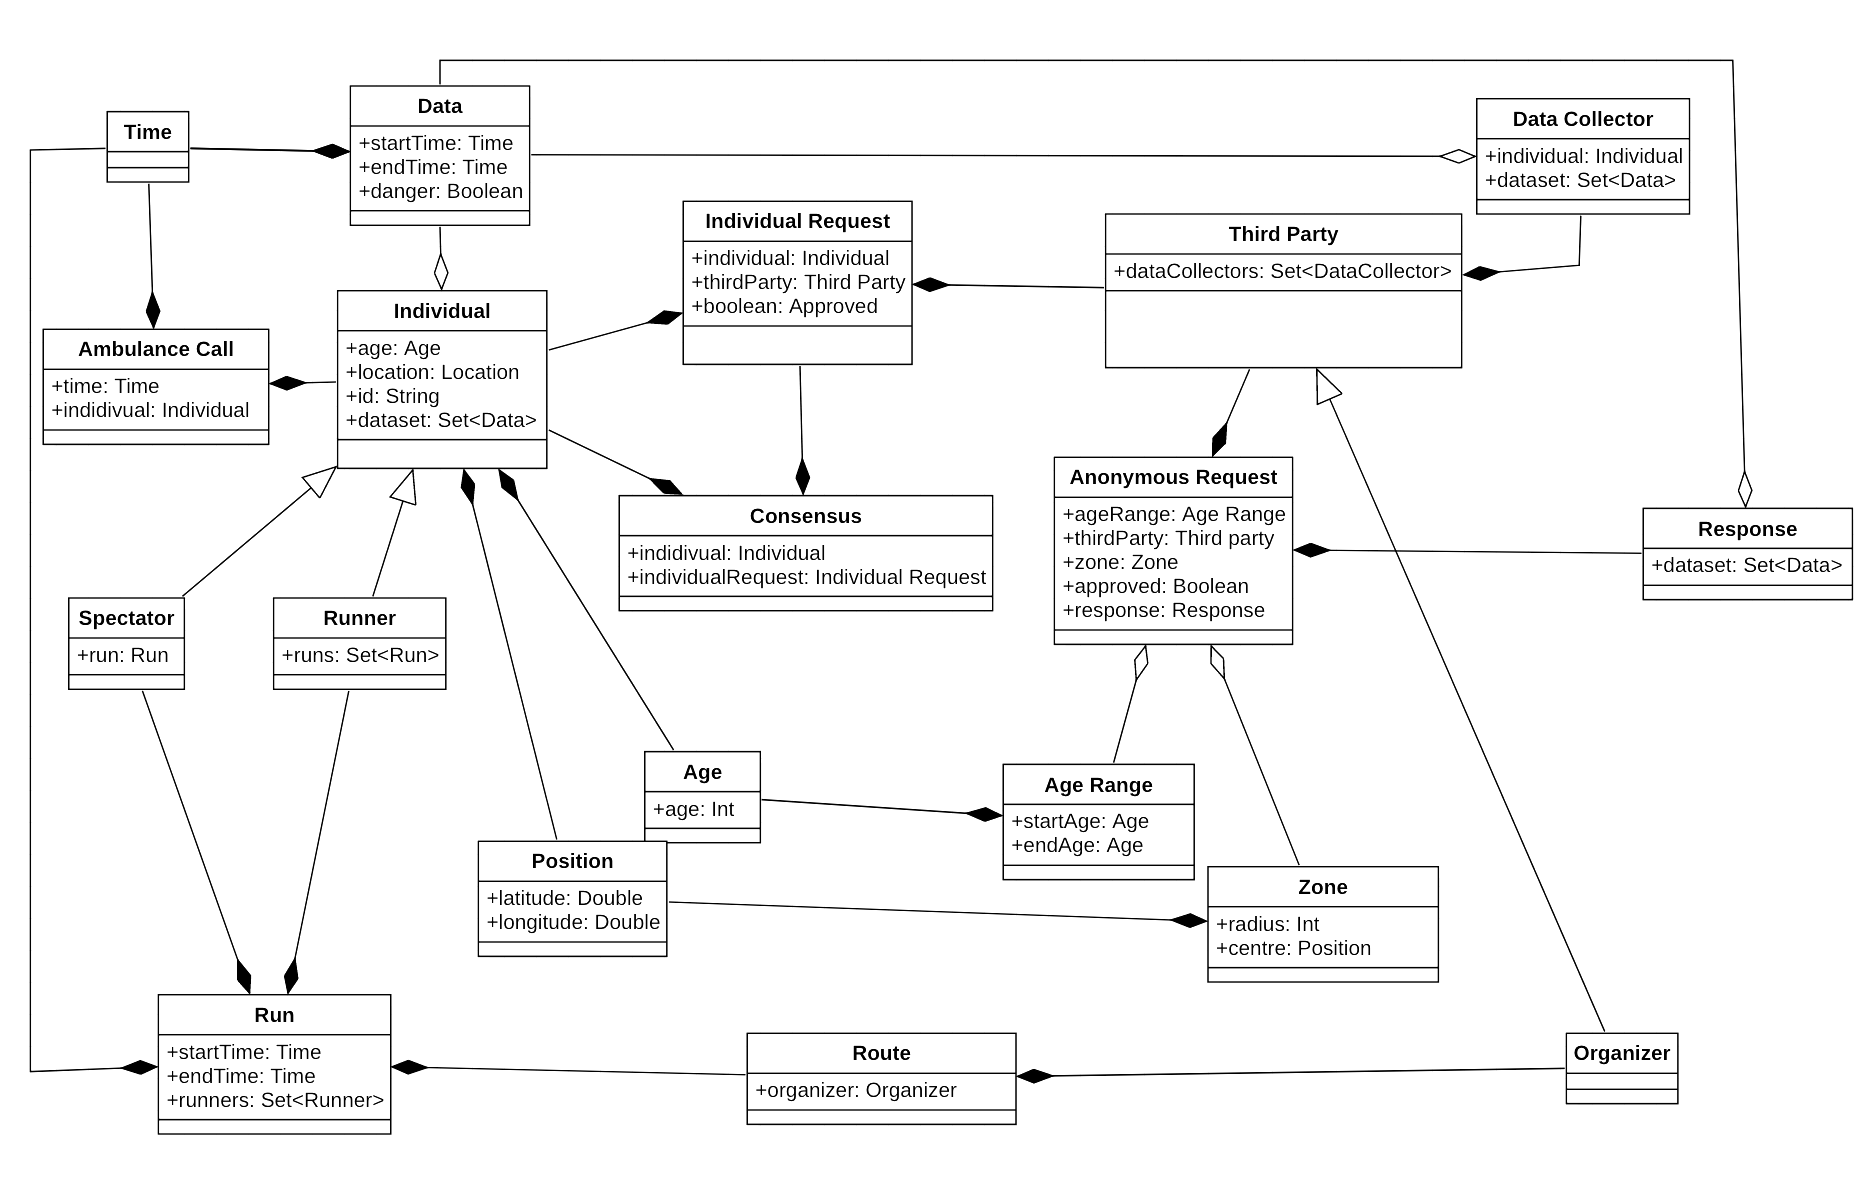
\includegraphics[width=\linewidth]{./images/UML1-0.png}
			\end{figure}
		\item \textit{Product functions} \\\\
		{\normalfont
In the following section, the functions of the system are listed and more precisely specified, with
respect to the already mentioned main services:
		\begin{itemize}
		\item Monitor an individual\\\\
		This function permits a third party (an association, an hospital, a company, etc) to ask for the data of a single user. More in detail, the third party can select a user by his/her SSN and send him/her a request to be allowed to access his/her data. If the user accepts it, then the third party will receive his/her data. The third party can request to keep monitoring the individual also after the request and it will receive the data as soon as they are ready. The user can decide to deny the permission at any moment. \\
		\item Request for anomymous aggregated data\\\\
		Third party can access anonymized data of a group of users enrolled in TrackMe. After a third party sends this kind of request by specifying some restrictions about users’ attributes, like age and residence, the system will collect the data of the target users, anonymize and send them to the third party if the number of users is greater than 1000 in order to guarantee the anonymity. The third party can request to keep receveing new data of the group after the request and it will receive the data as soon as they are ready until the group size will not be lower than 1000.\\
		\item SOS assistance\\\\
		The system keeps under control the health status of a user by monitoring the values of the health parameters acquired by external devices (smart watches or similar devices). If at least one of the parameters goes under a fixed threshold, the system generates an SOS within 5 seconds starting from the moment of the evaluation of the dangerous parameter. The SOS communicates to the ambulance the position of the user.\\
		\item Organize running events\\\\
		The system offers to a third party to organize a running event. The third party must specify the timing, the track and the maximum number of participants for the run.\\
		\item Enrol to runs or follow running events\\\\
		The user can select an available run and enrol to it by sending a simple request. Furthermore the system permits a user to track the position of the runners involved in a run. The user can check the list of available runs and, after selecting one among them, he/she can watch the map of the track filled up by points representing the runners in their actual position. \\
		\end{itemize}
		}
		\item \textit{User characteristics} \\\\
			{\normalfont
			Actors:\\
			\begin{itemize}
			 \item User: a registered individual who can use the TrackMe services. He/she can login to the system and then use all the functionalities provided by the platform.\\
			\item Third party: a registered entity that can use the TrackMe services. It can login to the system and then use all the functionalities provided by the platform.\\
 			\item System Manager:  an employee of TrackMe, in charge of the maintenance of the system. He/she does not need to be registered, since has been inserted in the system directly during the installation process.\\
			\end{itemize}
			}
		\item \textit{Assumptions, dependencies and constraints}\\
			\begin{legal}
    			\item Text assumptions\\
    			{\normalfont
				\begin{itemize}
					\item User can choose to disable AutomatedSOS service in preferences;\\\
					\item A SOS is sent through an SMS which contains the user's data and the coordinates of the position to be reached;\\\
					\item If the user is not able to connect the device, he/she can contact the TrackMe assistance by calling a specific number;\\
					\item When a user signs up to TrackMe he/she accpets also to treatment of his/her data for AutomatedSOS;\\
					\item The user can remove the consensus previously given to a third party.\\
				\end{itemize}}
			\newpage
			\item Domain assumptions \\
			{\normalfont
				\begin{itemize}
				\item D1) The measurements of the health status parameters of the individuals are supposed to be reliable;\\
				\item D2) The position of the individuals is supposed to be reliable;\\
				\item D3) The data acquired from the user’s devices are sent to the mobile application as soon as they are produced;\\
				\item D4) The identification data provided by the users are correct;\\
				\item D5) The identification data provided by the third parties are correct;\\
				\item D6) When an SOS is launched, an ambulance is sent to the position of the user linked to the account that raised the SOS itself;\\
				\item D7) The race takes place in an area with internet coverage and in a compliant track;\\
				\item D8) The location of a registered user is acquired by his smartphone used by the user himself;\\
				\item D9) Data related to the health status of a registered user are acquired by smartwatches or similar devices used by the user himself.\\
				\end{itemize}
			}
			\end{legal}
		\end{legal}
	
\newpage
	\item \underline{Specific requirements}
  		\begin{legal}
		\item \textit{External interface requirements}
			\begin{legal}
    		\item User interfaces \\\\
			\normalfont{
			In this section follow the main mockups that represent a basic idea of what the mobile app will look like in the first release:\\
			
						
					\begin{legal}
    					\item Login or Sign Up 
						\begin{figure}[H]
						\centering
  						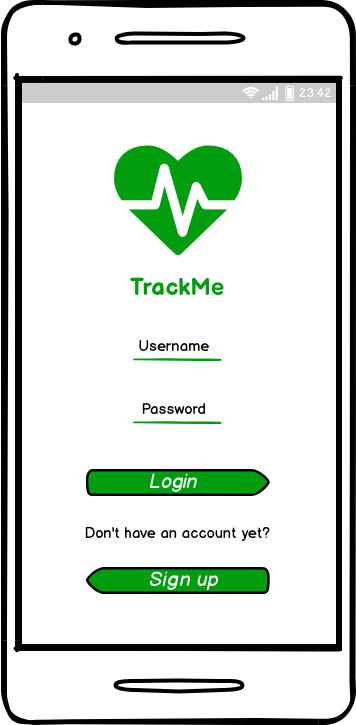
\includegraphics[scale=0.275]{./images/mockups/Login-Sign-up.png}
						\end{figure}
					\item  (a)Join a run - (b)Select the track of the run
						\begin{figure}[H]
						\centering
						\begin{subfigure}{.5\textwidth}
  						\centering
  						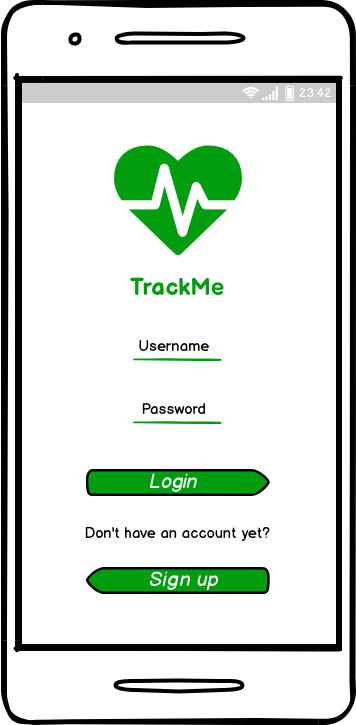
\includegraphics[width=.4\linewidth]{./images/mockups/Login-Sign-up.png}
 						 \caption{Join a run}
						\end{subfigure}%
						\begin{subfigure}{.5\textwidth}
 						 \centering
 						 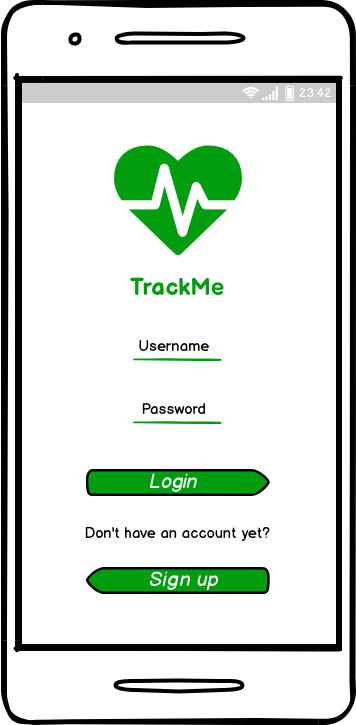
\includegraphics[width=.4\linewidth]{./images/mockups/Login-Sign-up.png}
 						 \caption{Select the track of the run}
						\end{subfigure}
						\end{figure}
					\newpage
					\item (a)Individual request  - (b)Group request
						\begin{figure}[H]
						\centering
						\begin{subfigure}{.5\textwidth}
  						\centering
  						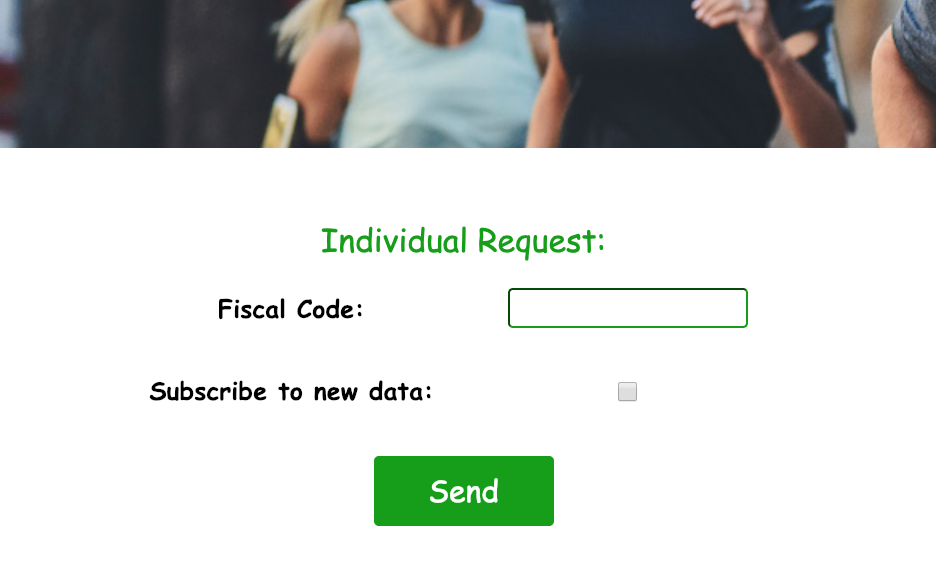
\includegraphics[width=.4\linewidth]{./images/mockups/Individual-request.png}
 						 \caption{Individual request}
						\end{subfigure}%
						\begin{subfigure}{.5\textwidth}
 						 \centering
 						 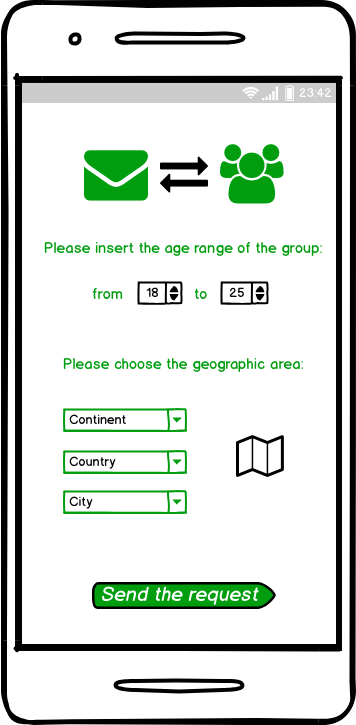
\includegraphics[width=.4\linewidth]{./images/mockups/Group-request.png}
 						 \caption{Group request}
						\end{subfigure}
						\end{figure}
				\end{legal}	
			}
			
			\item \textbf{Hardware interfaces}\\\\
This system is intended to stay with the user during his every day life. In order to guarantee the promised services, it’s necessary that users install the-front end application on a smartphone (Android or iOS) that can use GPS services to allow localization and supports Bluetooth in order to connect the device worn by the user to retrieve health data. This device can be a smartwatch or any other hardware able to get the interested health parameters.
Since the application must run over the internet, the smartphone is required to connect through WIFI or a wireless mobile telecommunications technology.\\
			\item \textbf{Software interfaces}\\\\
The application software doesn’t need to lean on other software in order to provide basic services, except for front-end application that must run on a operating system able to connect external devices like smartwatches. 
Meanwhile the service Track4Run requires to interact with a software that provides a map service which includes these functionalities:
				\begin{itemize}
				\item visualize a map on which a path that cross different points can be shown;
				\item draw in detail this path on the map;
				\item provide metrics and statistics about a point moving on the map.\\
				\end{itemize}
			\item \textbf{Communication interfaces}\\\\
The system is essentially split into a front-end and a back-end. They communicate over the internet network.
Furthermore a Bluetooth connection between smartphones and external devices is required.\\
			\end{legal}
		\newpage
    		\item \textit{Functional Requirements}
    		\begin{legal}
		\item Scenarios\\
		{\normalfont
		\begin{legal}
		\item \textbf{Join a run as a runner}\\

Mario is a sporty student who hears about a run organized by PoliMi Sport and would like to join it. PoliMi Sport is an association registered to TrackMe as a third party with the aim of guaranteeing the good health status of the enrolled students and proposing them new races every week. The unique way to join the run is to send the request to PoliMi Sport through the TrackMe app, so that Mario decides to download it and sign up. After that, he logs in with his credentials and looks for the run he is interested in. Once found, he asks to join that as a runner. Meanwhile system checks if the number of participants is not exceeded and if Mario has not already joined an overlapping run, then notifies Mario with the result.\\

		\item \textbf{Join a run as a spectator}\\

Luca is a professor who is fond of running and after a lecture hears his students talking about a run organized by the student union Poli4Run. It is an association registered to TrackMe as a third party with the aim of guaranteeing the good health status of the enrolled students and proposing them new races every week. He is very interested in the race joined by their students and he would like to go and see them competing, so Luca asks them for information and decides to follow their instructions. At first he downloads the TrackMe app and then he signs up. After that, he logs in with his credentials and looks for the run he is interested in. Once found, he asks to join that as a spectator. Meanwhile he system checks if the number of spectators is not exceeded and if Luca has not already joined an overlapping run, then notifies Luca with the result.\\

		\item \textbf{SOS launched}\\

Antonella is an old woman who had heart disease in the past so she would like to be daily monitored to avoid problems. Her young nephew tells her about the TrackMe app, through which she could fulfil her needs. Delighted by this kind of solution, she decides to buy a smartwatch and download the app. Then she signs up to the TrackMe app and checks to have the AutomatedSOS service correctly activated. One day, after having climbed the stairs, the app retrieves the data from her smartwatch and evaluates them as exceeding the danger thresholds, so that within 5 seconds the SOS is received by the medical facility that sends an ambulance to the position detected by the woman’s wearable device.\\


		\item \textbf{Individual request with a positive result}\\
 
The Green Hospital wants to monitor the health status of one of its patient, Paolo, who recently recovered from an important disease. The hospital knows the mobile application TrackMe and it already has a valid account on the app. The doctor who is taking care of Paolo asks him to download the application, to link a smart device able to measure the health parameter needed by the doctor to monitor his health status and to register to the service. The doctor, using the account of the hospital, sends a request to Paolo (known by his SSN) for the treatment of his data. Paolo accepts the request and the hospital is allowed to receive the data produced by Paolo’s device.\\

		\item \textbf{Anonymous request with a negative result}\\

The association WalkMore wants to promote walking among young people who have a too sedentary life. As a first step to reach its goal WalkMore decides to use the new amazing app Data4Help to monitor the distance that a group of target young people runs every day. WalkMore registers to Data4Help and forwards a request to access the anonymized data of people between 18 and 23 living in the municipality of Milan. Unfortunately, due to the recent release of the application, there is not enough data in order to guarantee the privacy of the selected target and the request is frozen until enough data are collected.  \\

		\end{legal}
		}
    		\item Use Case Diagram\\\\
		\normalfont{
		Here follows the representation of the users interaction with the system.\\
		}
    			\begin{figure}[H]
			  	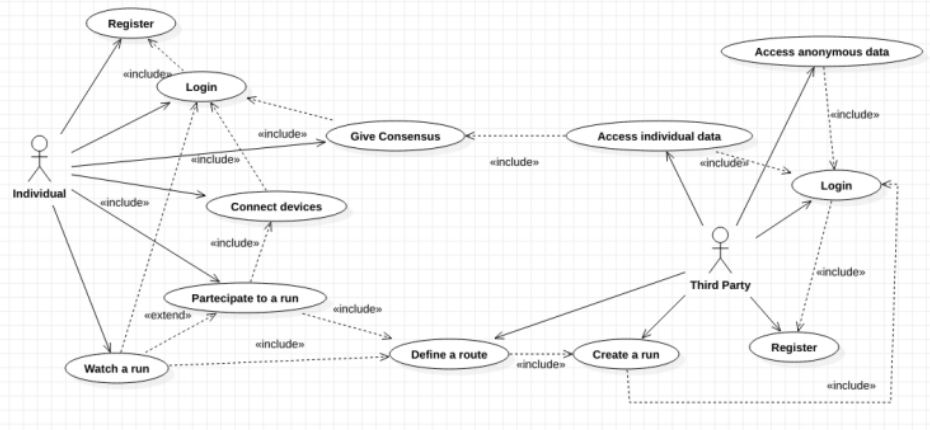
\includegraphics[width=\linewidth]{./images/usecase.png}
				\end{figure}
				\item \textbf{Use Cases Descriptions}\\\\
				%SIGN UP
				\begin{tabular}{| m{3.5cm} | m{8cm}| }
				\hline
					Name & Sign up\\
				\hline
					Actor & Individual\\
				\hline
					Entry Conditions & Application installed
				on his device.\\
				\hline
					Event Flows & \begin{enumerate}
									\item The user opens the application.
									\item The user goes to the sign up section.
									
									\item The user gives all the necessary informations.
									\item The user chooses an username and a password.
									\item The user confirms his operations.
									\item The system save informations.
				\end{enumerate}\\
				\hline
					Exit Conditions & The user is successfully  registered and now he's able to log in.\\
				\hline
					Exceptions & \begin{enumerate}
									  \item The user is already registered.
									  \item The informations are incorrect or
									   missing.
				\end{enumerate}
				The user is notified and invited to try again.\\
				\hline
				\end{tabular}\\
				\\\\\\
				%LOGIN
				\begin{tabular}{| m{3.5cm} | m{8cm}| }
				\hline
					Name & Login\\
				\hline
					Actor & Individual\\
				\hline
					Entry Conditions & The user is previously successfully registered and has the application installed
				on his device.\\
				\hline
					Event Flows & \begin{enumerate}
									  \item The user opens the application.
									  \item The user goes to the login section.
									  \item The user inserts username and password.
									  \item The system checks if the credentials are correct.
				\end{enumerate}\\
				\hline
					Exit Conditions & The user is successfully logged in and he can access all the services. \\
				\hline
					Exceptions & The credentials are incorrect. The user is notified and invited to try again.\\
				\hline
				\end{tabular}\\\\\\
				%CONNECT A DEVICE
				\begin{tabular}{| m{3.5cm} | m{8cm}| }
				\hline
					Name & Connect a device\\
				\hline
					Actor & Individual\\
				\hline
					Entry Conditions & User already logged in.\\
				\hline
					Event Flows & \begin{enumerate}
									\item The user goes to the preference section.
									\item The user chooses to connect a device and then selects the right one.
				\end{enumerate}\\
				\hline
					Exit Conditions & The device is successfully connected to the application.\\
				\hline
					Exceptions & The system is not able to find or connect the device. The user is notified and invited to try again by reading carefully the connection instructions or to contact the help assistance of TrackMe.\\
				\hline
				\end{tabular}\\
				\\\\\\
				%WATCH A RUN
				\begin{tabular}{| m{3.5cm} | m{8cm}| }
				\hline
					Name & Watch a run\\
				\hline
					Actor & Individual\\
				\hline
					Entry Conditions & User already logged in.\\
				\hline
					Event Flows & \begin{enumerate}
									\item The user goes to the run section.
									\item The user chooses the run he wants to watch.
									\item The system screens a map with the route and the partecipants.
									\item The user can choose to watch statistics.
									\item If the user chooses to watch statistics the system provides him details about the run.
				\end{enumerate}\\
				\hline
					Exit Conditions & The user is able to follow a run.\\
				\hline
					Exceptions & There are no current runs. The user is notified with the list of incoming runs.\\
				\hline
				\end{tabular}\\
				\\\\\\
				%PARTECIPATE TO A RUN
				\begin{tabular}{| m{3.5cm} | m{8cm}| }
				\hline
					Name & Partecipate to a run\\
				\hline
					Actor & Individual\\
				\hline
					Entry Conditions & User already logged in and he has already given the consensus to the third party.\\
				\hline
					Event Flows & \begin{enumerate}
									\item The user goes to the run section.
									\item The system lists all available incoming runs which don't overlap with other user's runs.
									\item The user selects an incoming run.
									\item The system save the choice of the user in his calendar events.
				\end{enumerate}\\
				\hline
					Exit Conditions & The user is a official partecipant of the run and he will be notified some days before the run.\\
				\hline
					Exceptions & There are no available runs. The user is asked if he wants to be notified as soon as a new run is available.\\
				\hline
				\end{tabular}\\
				\\\\\\
				%GIVE CONSENSUS
				\begin{tabular}{| m{3.5cm} | m{8cm}| }
				\hline
					Name & Give consensus\\
				\hline
					Actor & Individual\\
				\hline
					Entry Conditions & User already logged in and a third party has requested access to user data.\\
				\hline
					Event Flows & \begin{enumerate}
									\item The user goes to the preference section.
									\item The user chooses to give or not the consensus to the third party.
									\item The system saves user's choice and sends it to the third party.
				\end{enumerate}\\
				\hline
					Exit Conditions & The third party can access user data if and only if the user gave the consensus.\\
				\hline
				\end{tabular}\\
				\\\\\\
				%CREATE A RUN
				\begin{tabular}{| m{3.5cm} | m{8cm}| }
				\hline
					Name & Create a run\\
				\hline
					Actor & Third Party\\
				\hline
					Entry Conditions & Third party logged in.\\
				\hline
					Event Flows & \begin{enumerate}
									\item The third party goes to the organize a run section.
									\item The system show to third party all the incoming events
									\item The third party chooses to create a run.
									\item The third party inserts all the relevant information except the route, it can be define later on.
									\item The system saves the event and update the calendar of incoming events of all the users.
				\end{enumerate}\\
				\hline
					Exit Conditions & The third party is ready to define a route and all the users are informed about the run.\\
				\hline 
					Exceptions & If the user hasn't given all the informations, he's asked to provide the missing ones.
					\\
				\hline
				\end{tabular}\\
				\\\\\\
				%ACCESS INDIVIDUAL DATA
				\begin{tabular}{| m{3.5cm} | m{8cm}| }
				\hline
					Name & Access individual data\\
				\hline
					Actor & Third Party\\
				\hline
					Entry Conditions & Third party logged in.\\
				\hline
					Event Flows & \begin{enumerate}
									\item The third party goes to the individual request section.
									\item The third party inserts the social security number of a person in order to request access of his/her data.
									\item The system forwards the request to the individual.
				\end{enumerate}\\
				\hline
					Exit Conditions & The user is notified about the request of the third party.\\
				\hline
					Exceptions & \begin{enumerate}
					\item The third party has already requested to access the data of the individual. In this case the third party is informed about the status of the individual's response.
					\item The social security number is not correct. The third party is notified and asked to try again.
					\end{enumerate}\\
				\hline
				\end{tabular}
				\\\\\\
				%ACCESS ANONYMOUS DATA
				\begin{tabular}{| m{3.5cm} | m{8cm}| }
				\hline
					Name & Access anonymous data\\
				\hline
					Actor & Third Party\\
				\hline
					Entry Conditions & Third party logged in.\\
				\hline
					Event Flows & \begin{enumerate}
									\item The third party goes to the group request section.
									\item The third party inserts the values of attributes of the the group of which is interested in.
									\item The system checks if the group is big enough to guarantee anonymity.
									\item The system will send the data to third party as soon as they are ready.
				\end{enumerate}\\
				\hline
					Exit Conditions & The third party has got access to the data of the interested group.\\
				\hline
					Exceptions & If the group is not big enough, the third party is notified and asked to try with other values of attributes.\\
				\hline
				\end{tabular}
				\\\\\\
			\newpage
			\item \textbf {Diagrams}\\\\
			{\normalfont
			In this section follow the interaction diagrams that detail how the main TrackMe operations are carried out by the software system:\\
			
			\begin{legal}
			
			\item Login - \textit{ Sequence diagram}
				\begin{figure}[H]
				\center
  				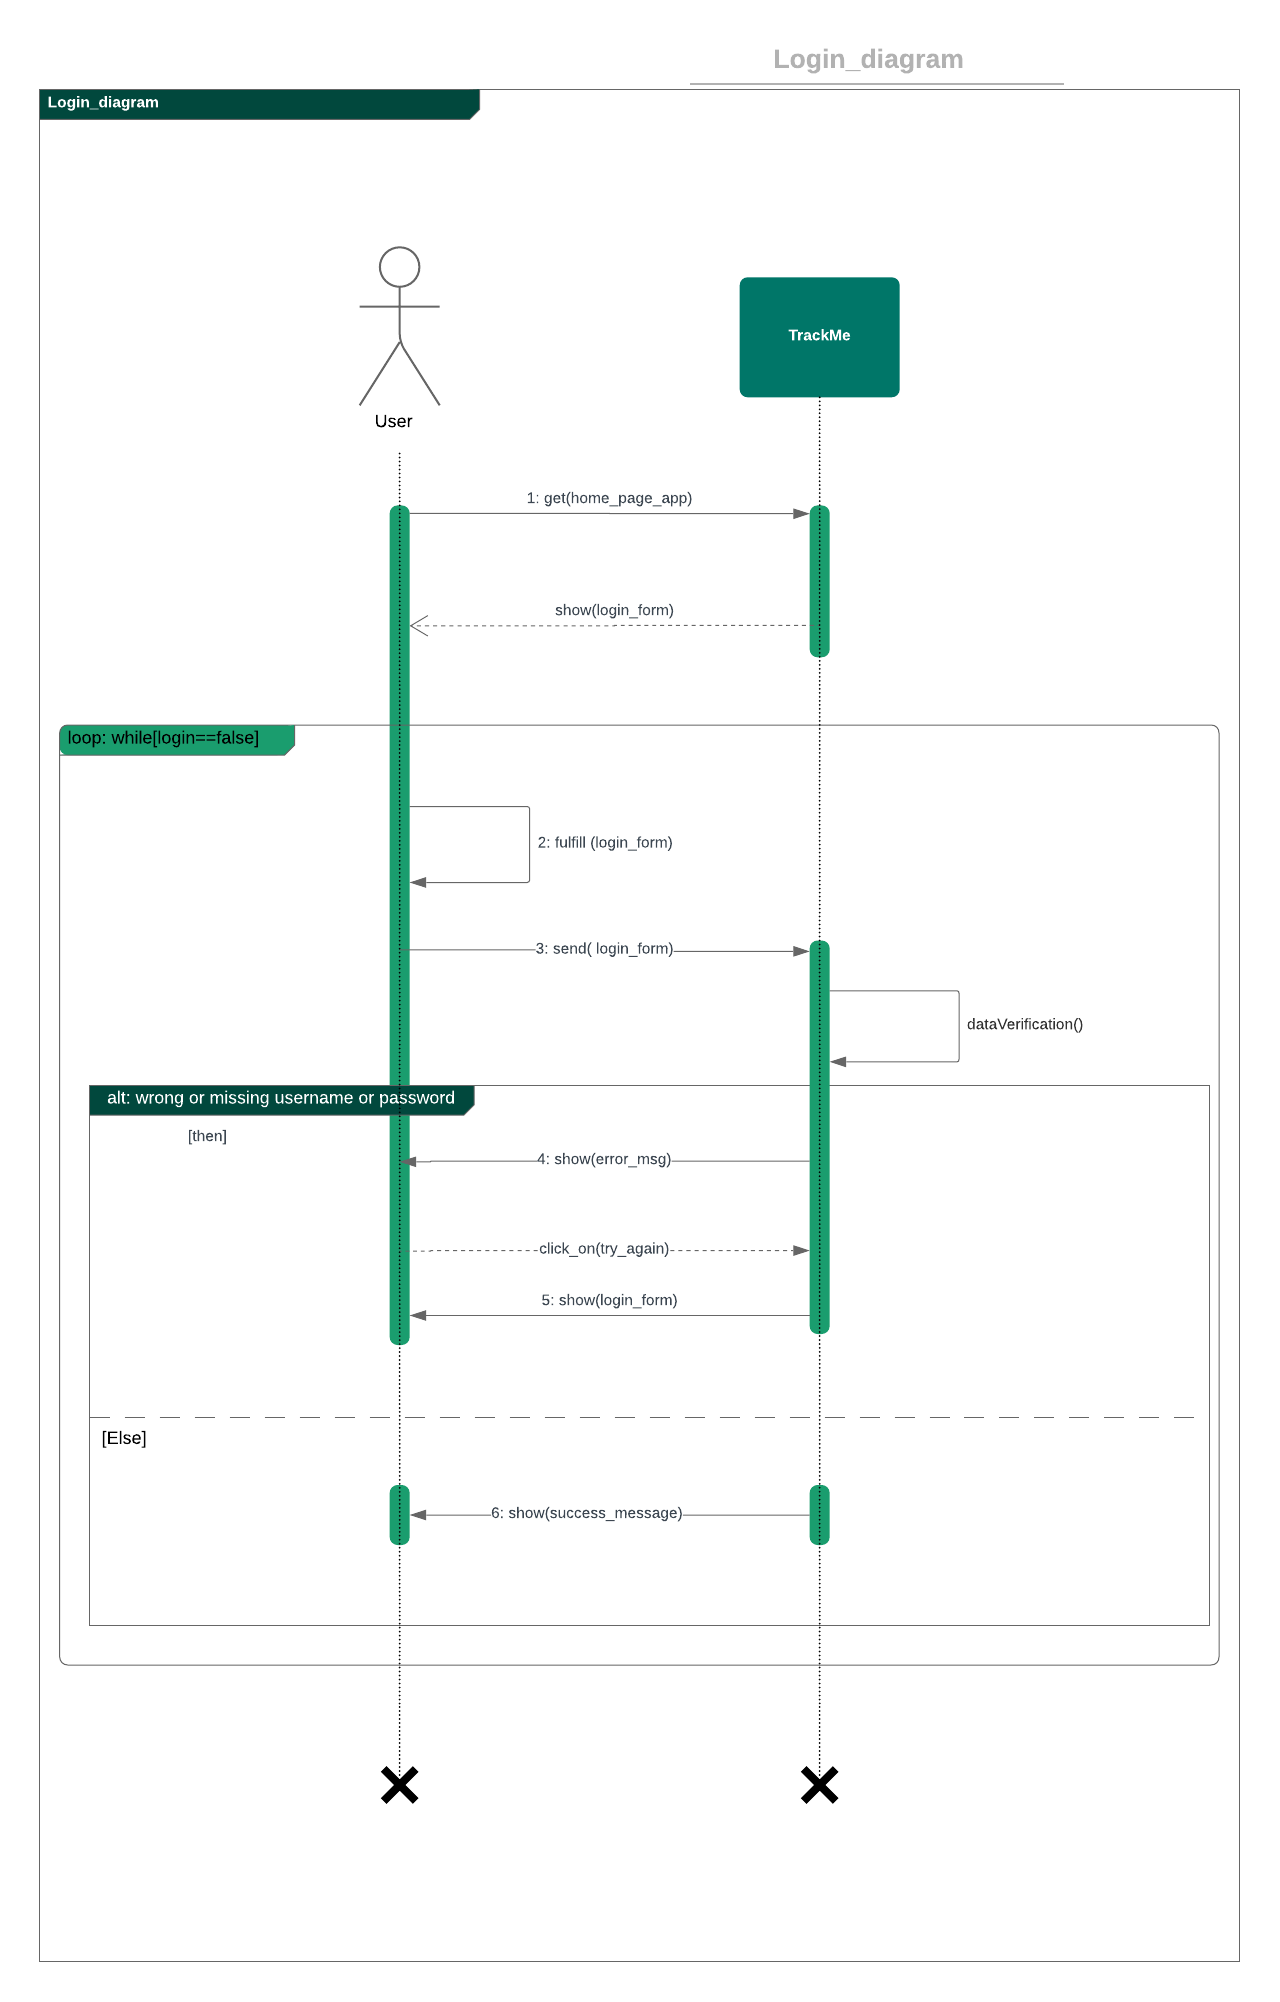
\includegraphics[width=160mm]{./images/seq-diagrams/Login_diagram.png}
				\end{figure}
			\newpage
			\item Sign up - \textit{ Sequence diagram}
				\begin{figure}[H]
				\center
  				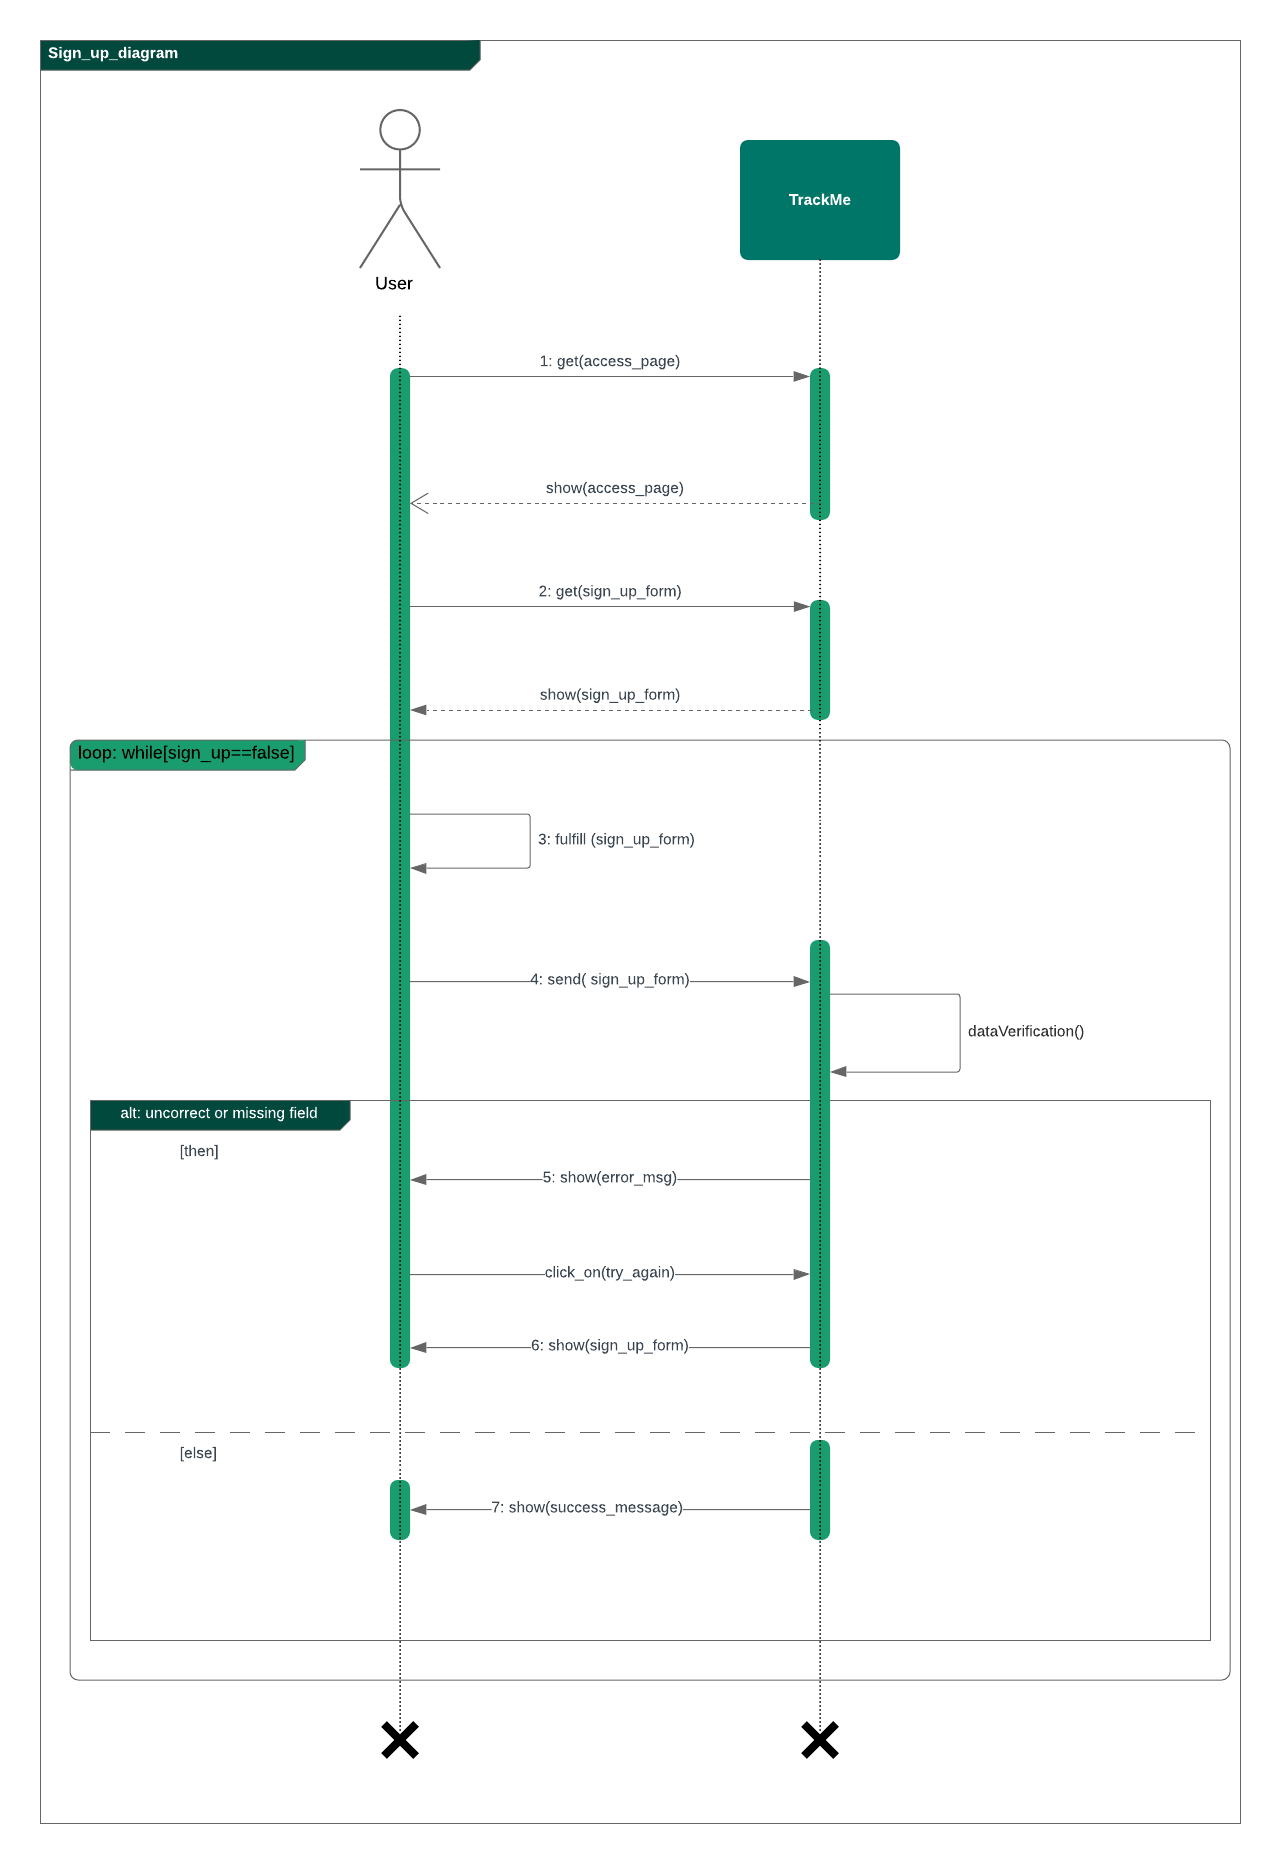
\includegraphics[width=160mm]{./images/seq-diagrams/Sign_up_diagram.png}
				\end{figure}
			\newpage
			\item Individual request - \textit{ Sequence diagram}
				\begin{figure}[H]
				\center
  				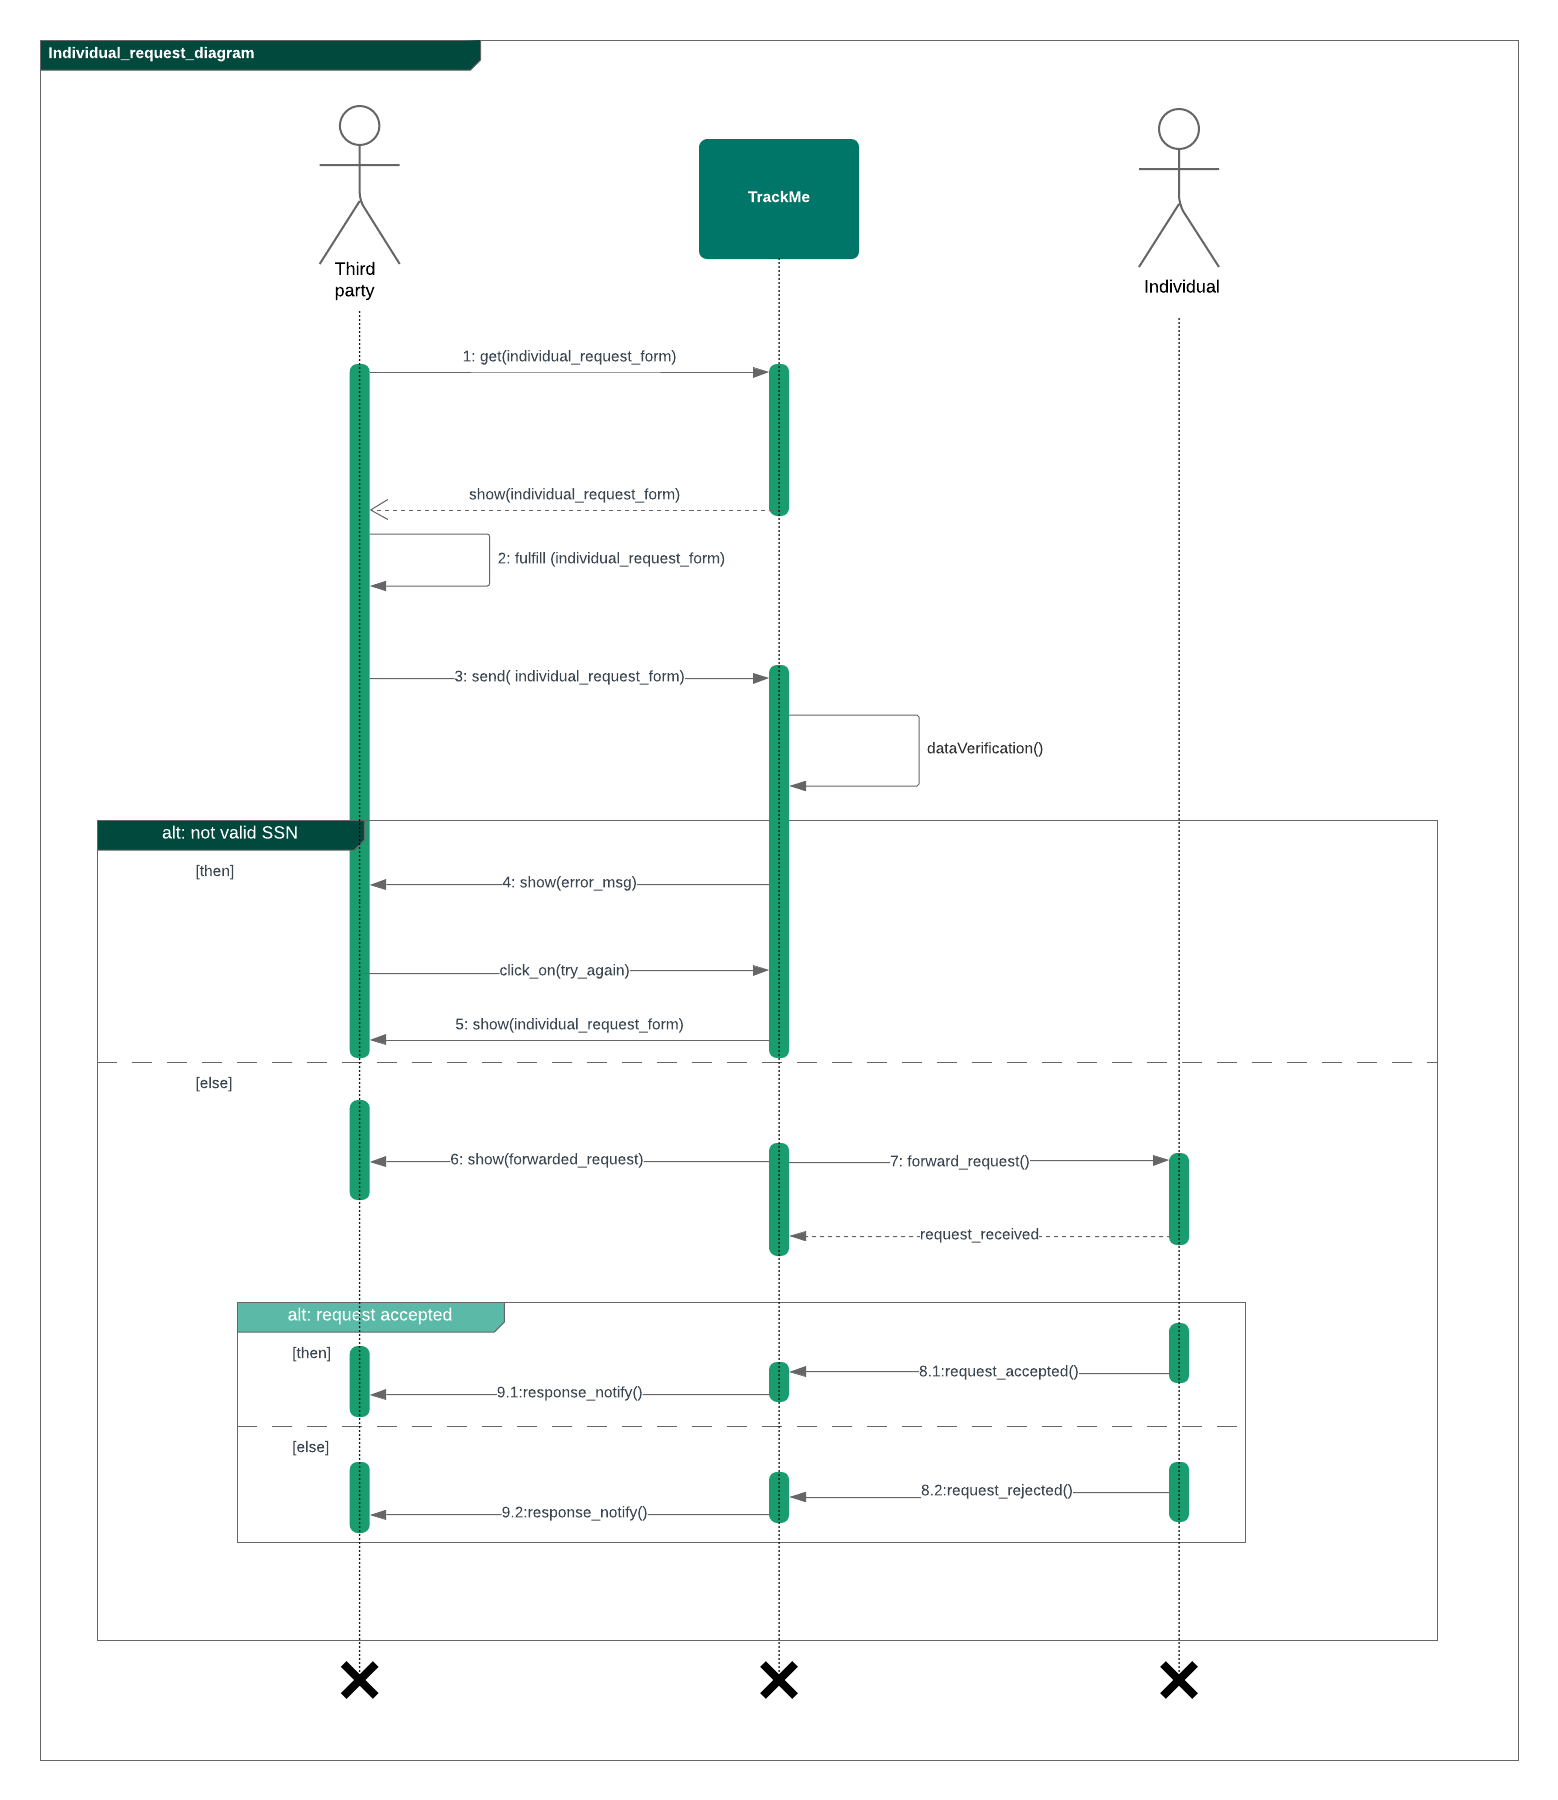
\includegraphics[width=160mm]{./images/seq-diagrams/Individual_request_diagram.png}
				\end{figure}
			\newpage	
			\item Group request - \textit{ Sequence diagram}
				\begin{figure}[H]
				\center
  				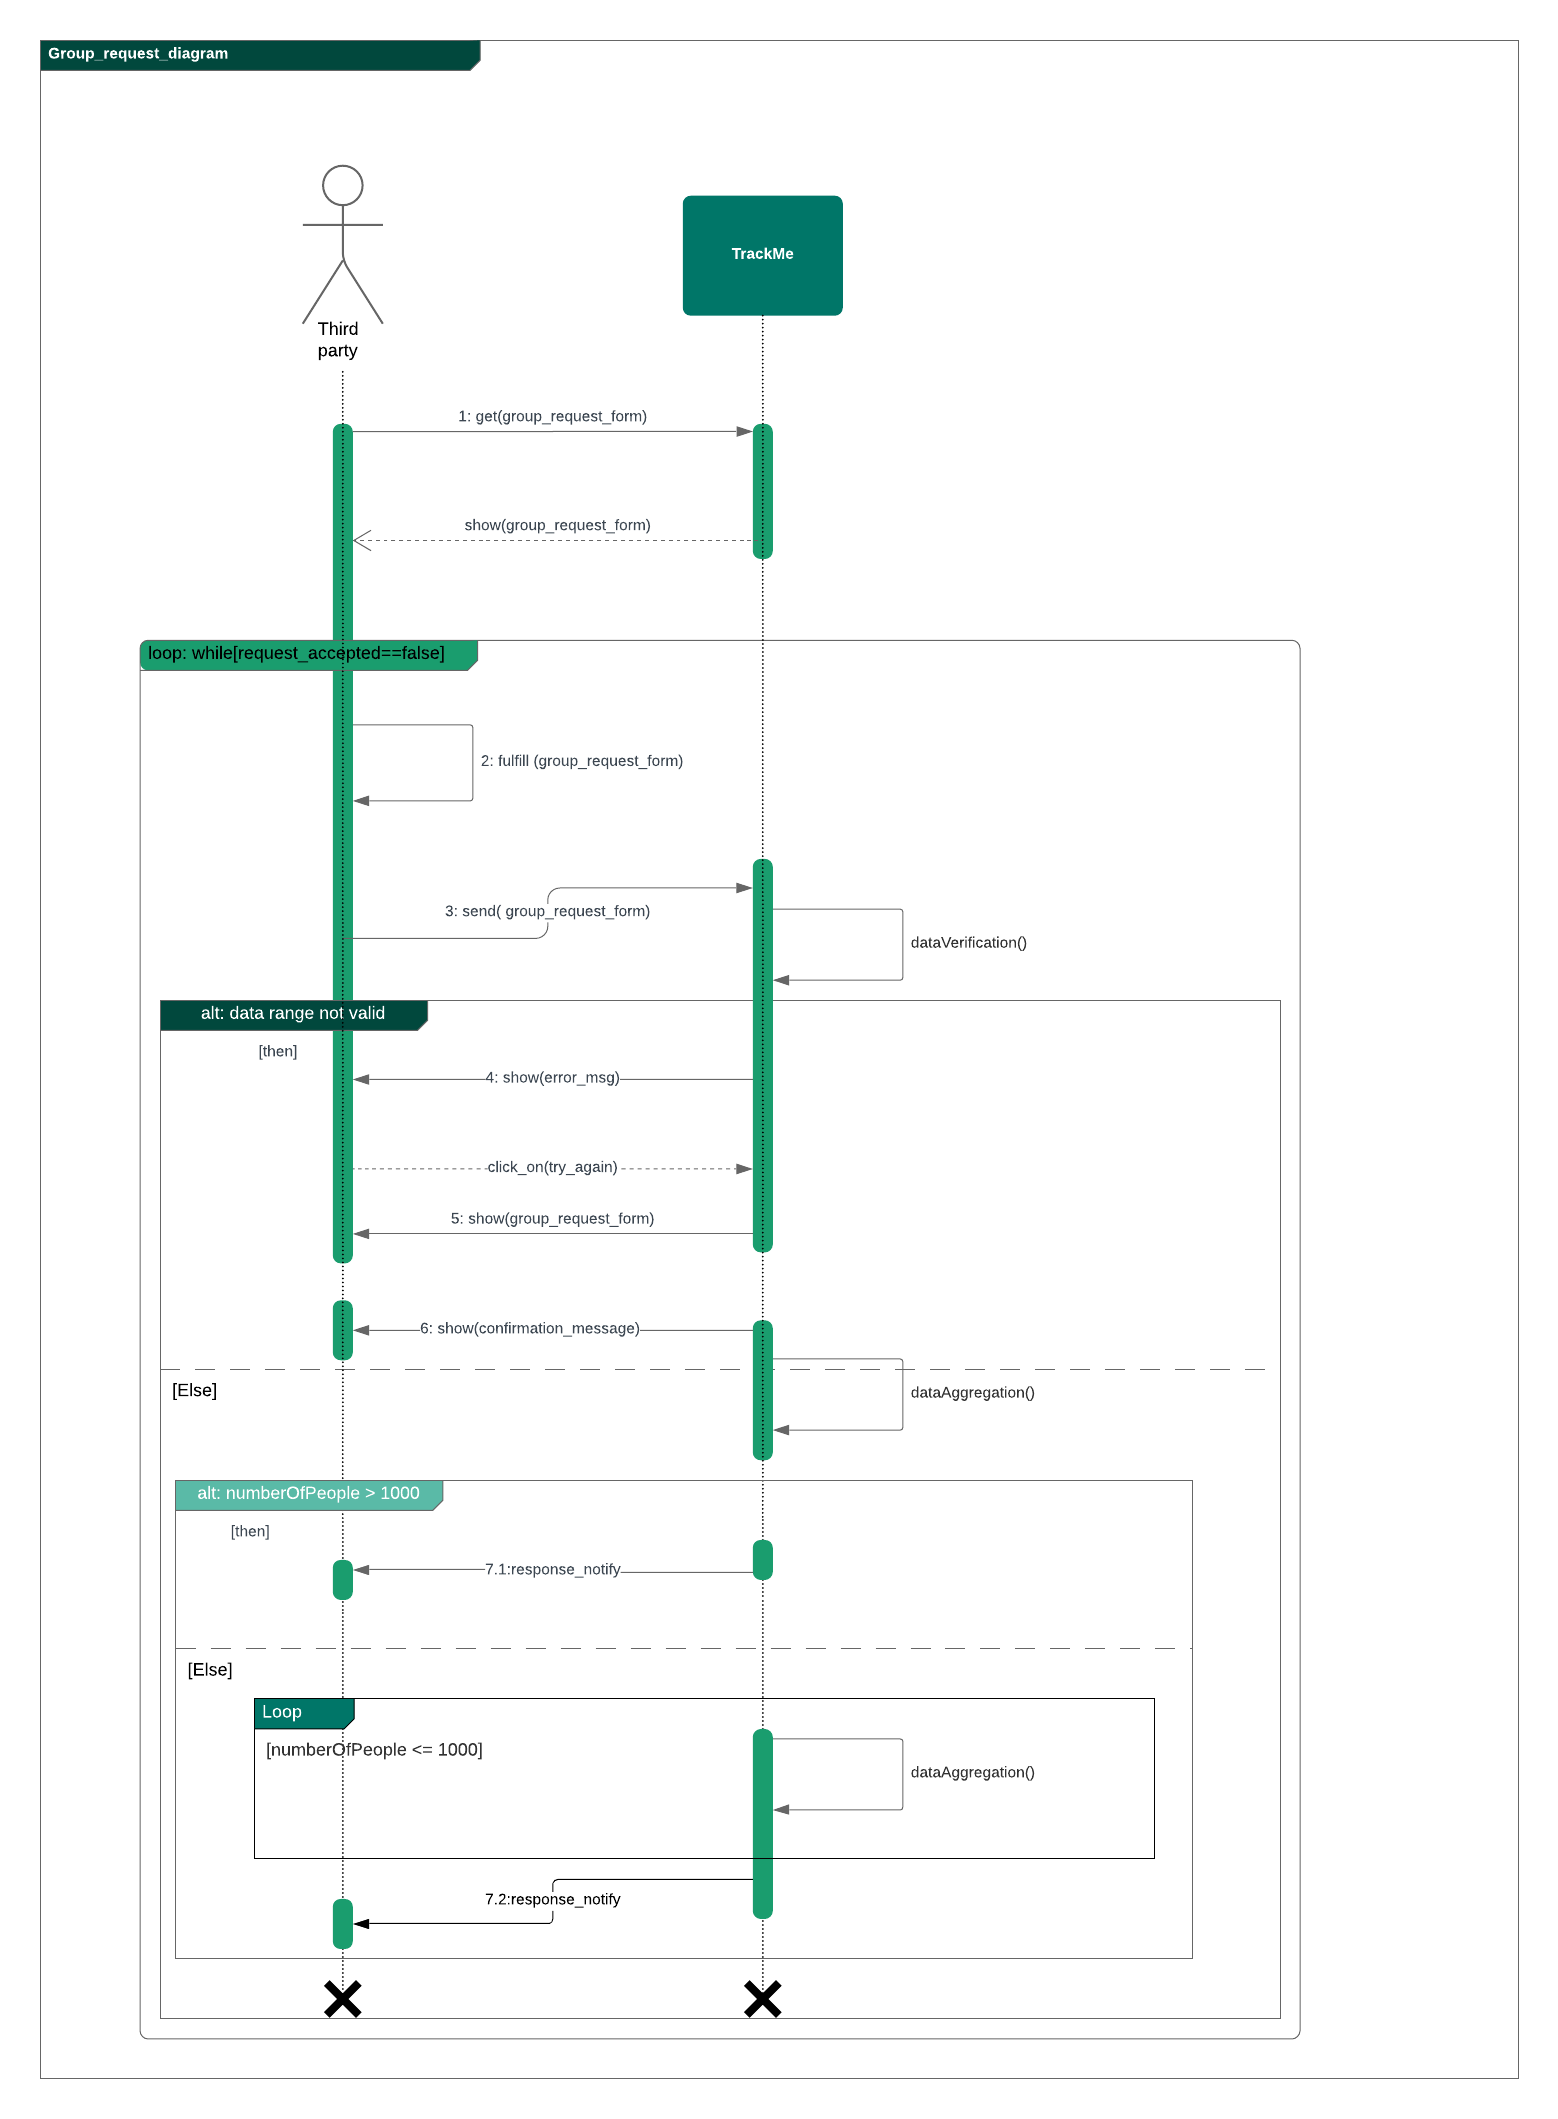
\includegraphics[width=160mm]{./images/seq-diagrams/groupRequest.png}
				\end{figure}
			\newpage	
			\item Join a run  - \textit{ Sequence diagram}
				\begin{figure}[H]
				\center
  				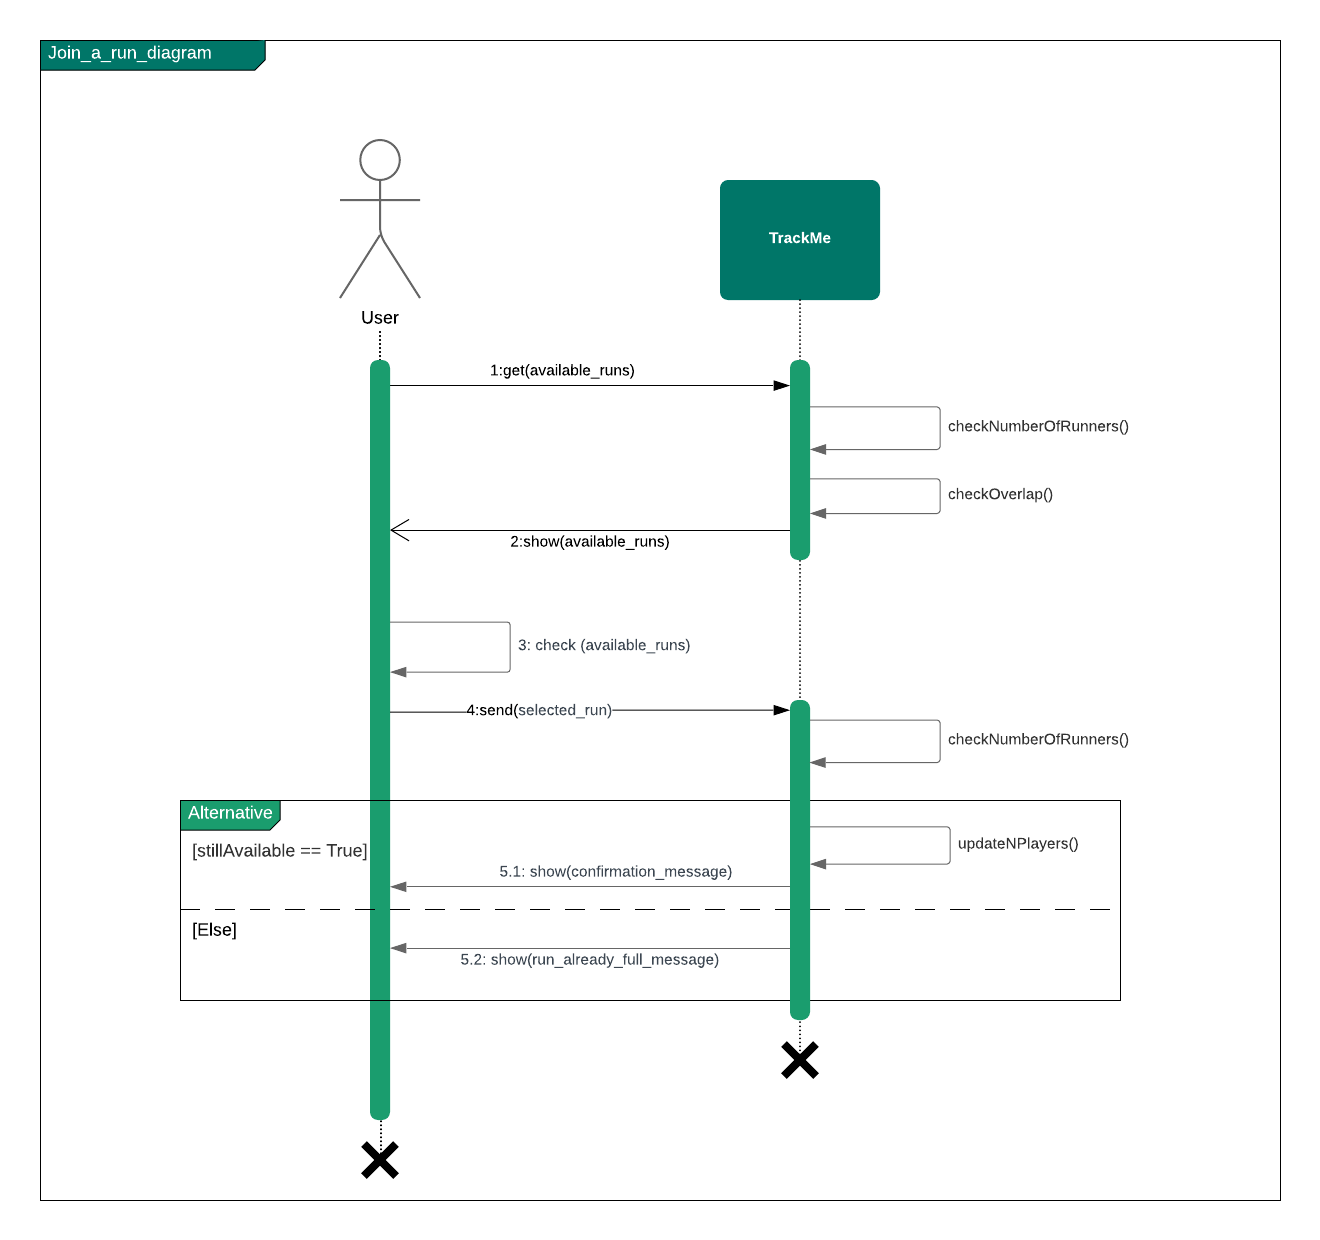
\includegraphics[width=160mm]{./images/seq-diagrams/joinARun.png}
				\end{figure}
			\newpage	
			\item Organize a run - \textit{ Sequence diagram}
				\begin{figure}[H]
				\center
  				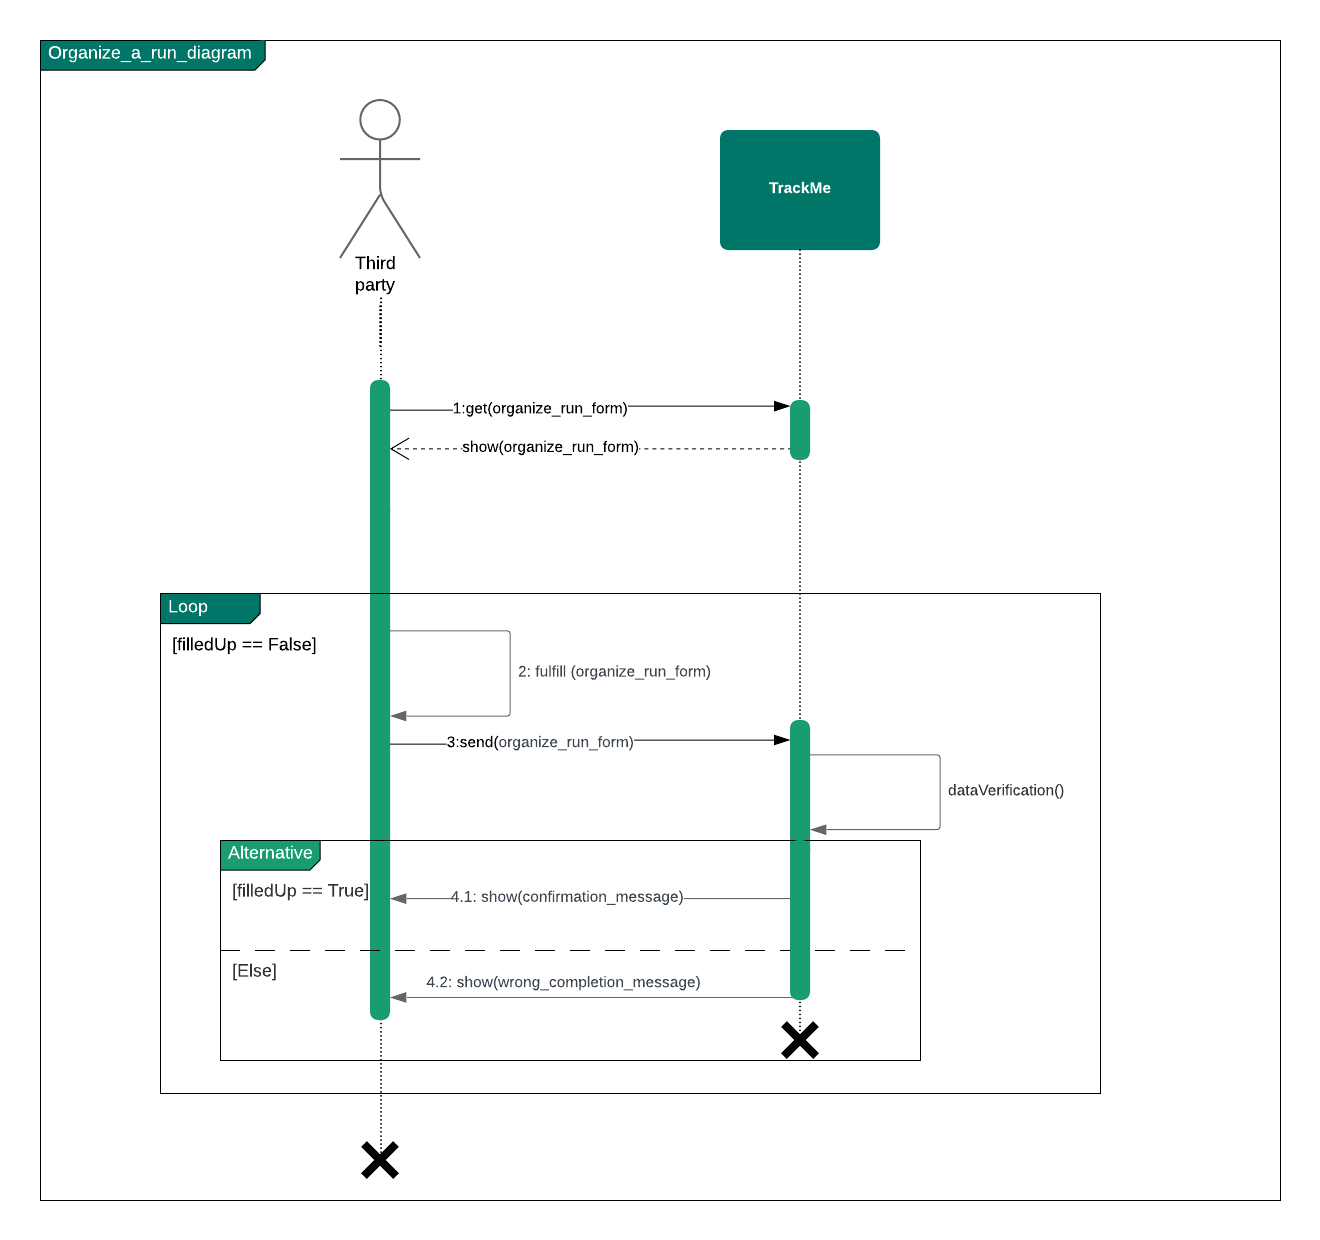
\includegraphics[width=160mm]{./images/seq-diagrams/organizeARun.png}
				\end{figure}
			\newpage	
			\item Join a run  - \textit{ Activity diagram}
				\begin{figure}[H]
				\center
  				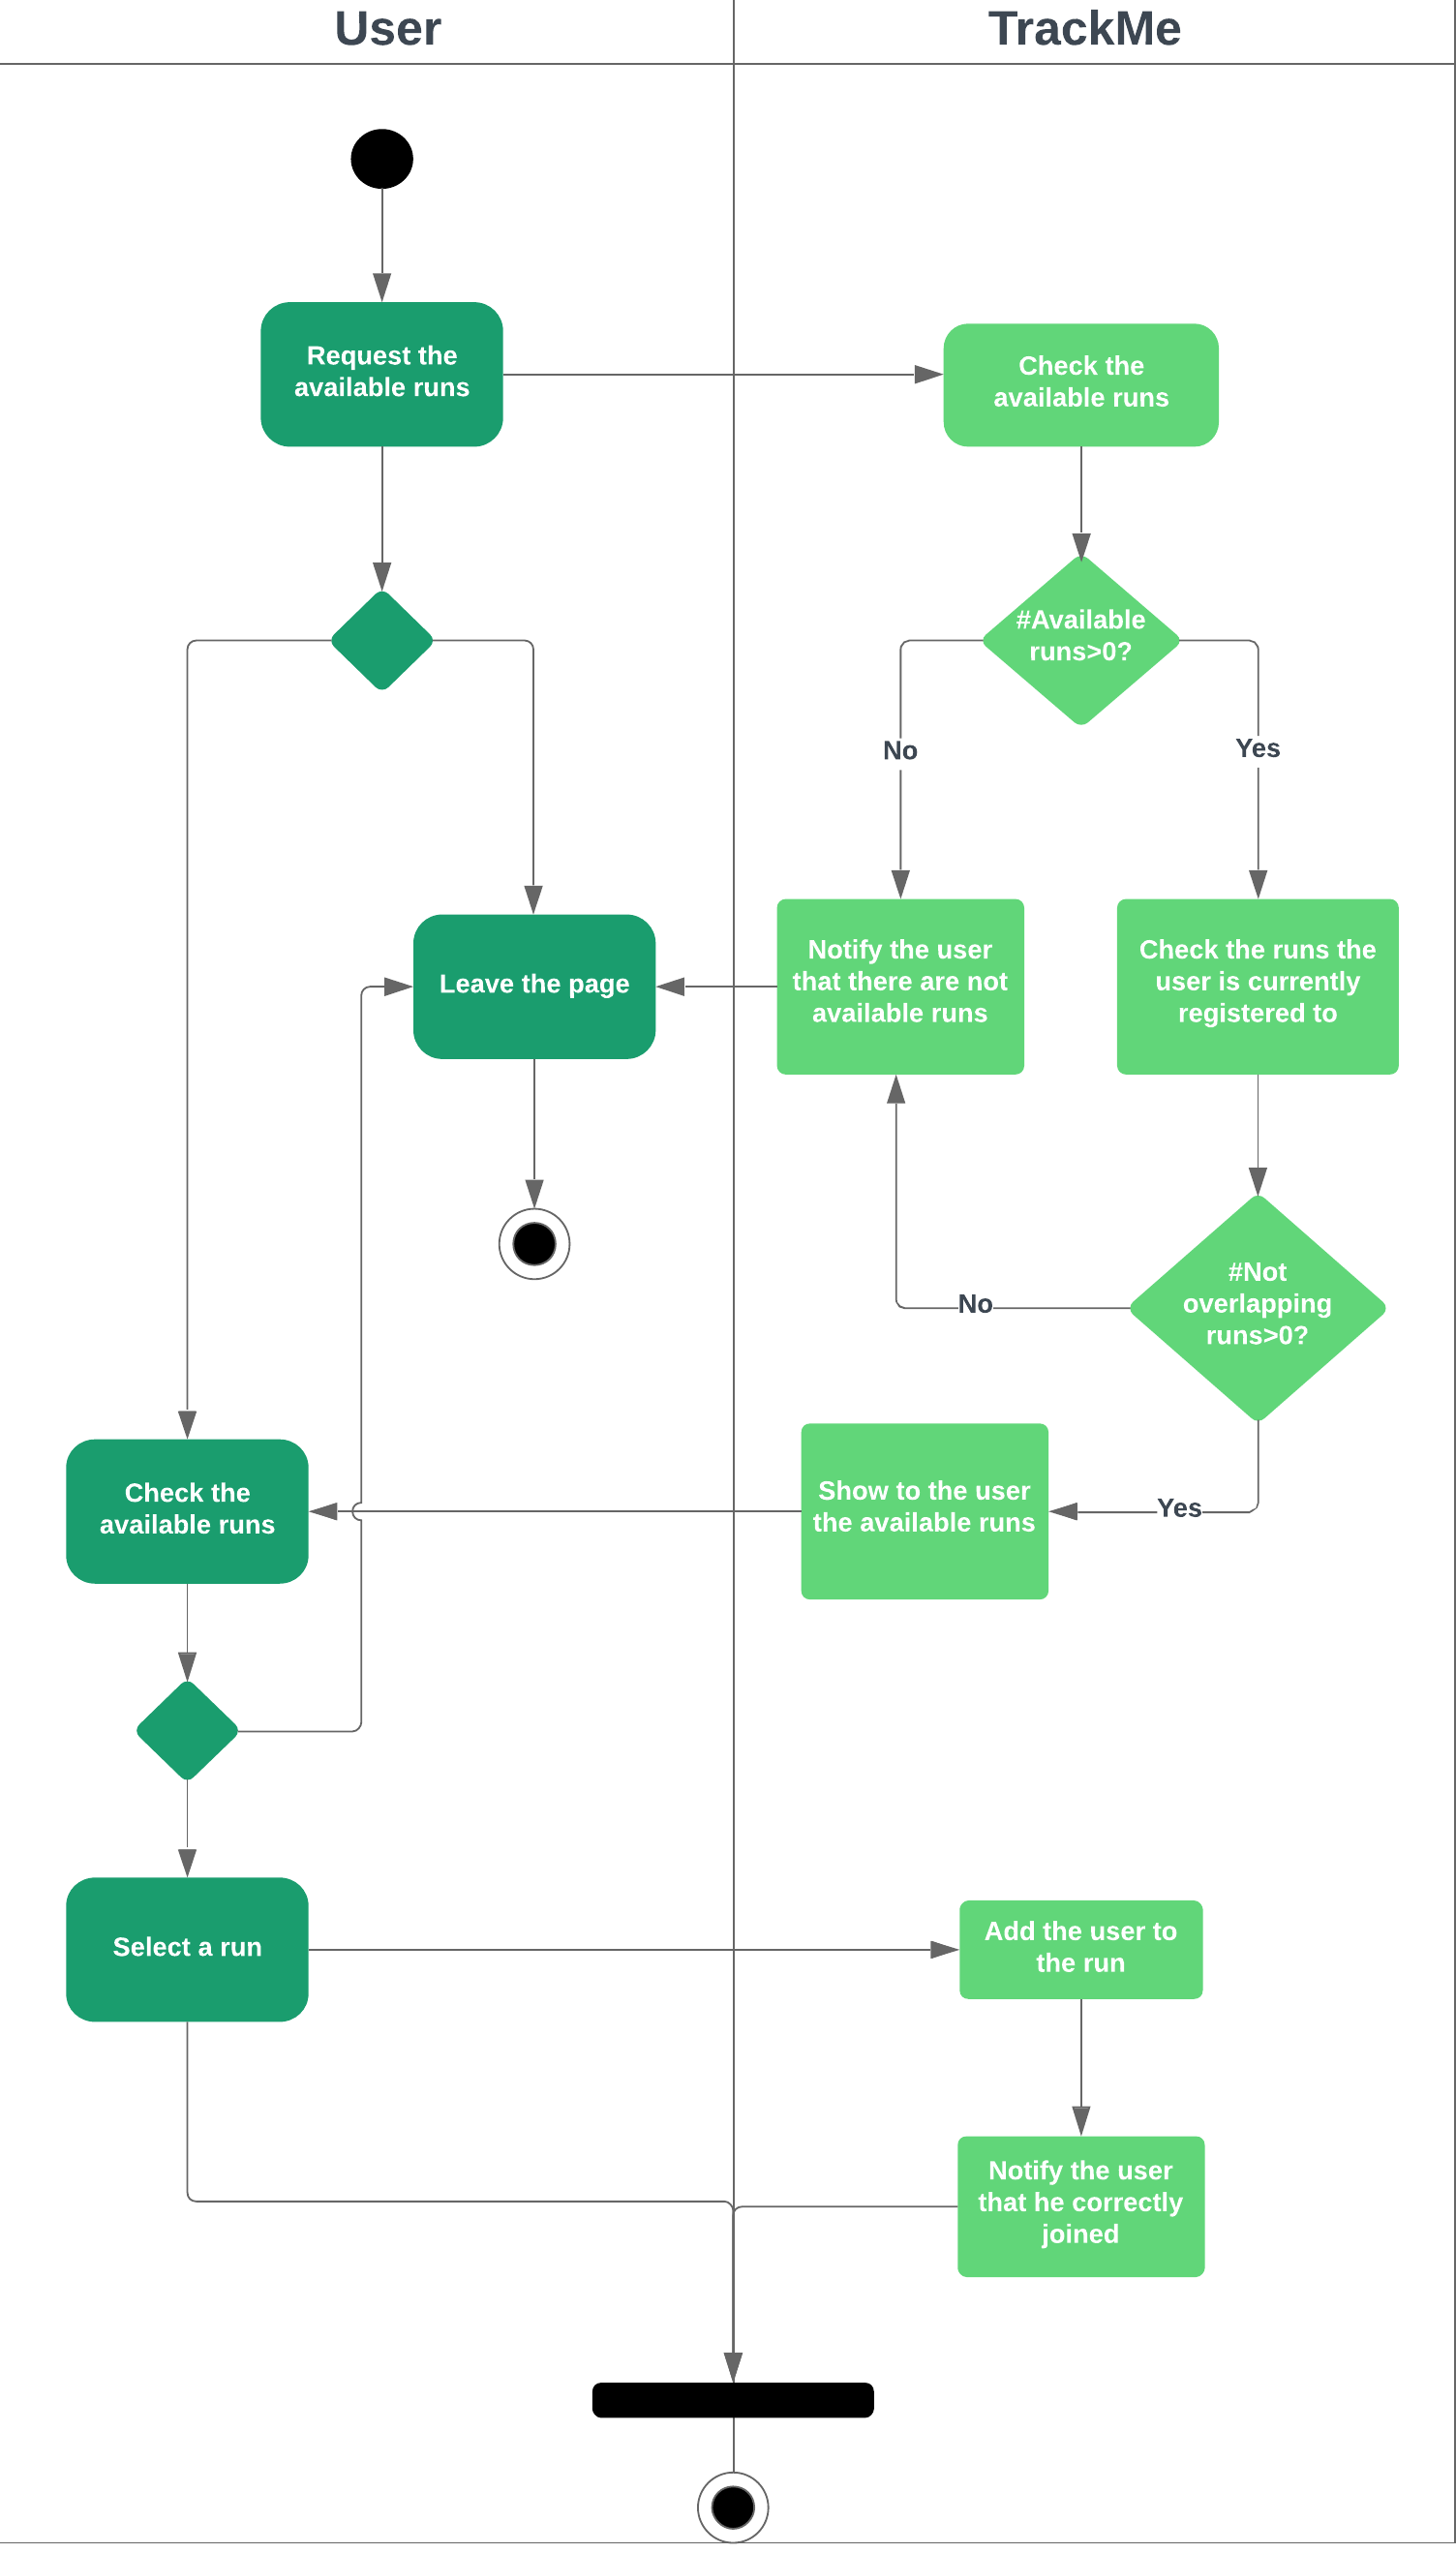
\includegraphics[width=120mm]{./images/Join-a-run-activity-diag.png}
				\end{figure}
			\newpage
			\end{legal}
			}
    		
			
			% Requirements --------------
			\item \textit{Global requirements}\\
			\begin{itemize}
				\normalfont{
				\item Third parties and individuals must have registered and logged in to use the services;\\
				\item The app is able to acquire data and to share data with the servers also in background in users' smartphones;\\
				\item There must be a fully working connection between the application and the smartwatches or similar devices.\\
				}
			\end{itemize}
			\item \textit{Mapping on requirements}\\
				\begin{itemize}
				\item G1) Third parties can monitor the position and the health status of the individuals;\\
				{\normalfont
					\begin{itemize}
					\item D1) The measurements of the health status parameters of the individuals are supposed to be reliable;\\
	 				\item D2) The position of the individuals is supposed to be reliable;\\
					\item D8) The location of a registered user is acquired by his smartphone used by the user himself;\\
					\item D9) Data related to the health status of a registered user are acquired by smartwatches or similar devices used by the user himself;\\
					\item R1) The users must have given the consensus to the treatment of their information to the third party;\\
					\item R2) The system must be able to provide to the third party the location and the health status of individuals;
					\item R3) The system must be able to retrieve data from the smartwatches and similar devices;\\
					\item R27) The system must be able to store data retrieved from registered users;\\
					\end{itemize}
				}
				\item G2) Third parties can access the anonymized data of the groups of individuals;\\
				{\normalfont
					\begin{itemize}
					\item D1) The measurements of the health status parameters of the individuals are supposed to be reliable;\\
	 				\item D8) The location of a registered user is acquired by his smartphone used by the user himself;\\
					\item D9) Data related to the health status of a registered user are acquired by smartwatches or similar devices used by the user himself;\\
					\item R3) The system must be able to retrieve data from the smartwatches and similar devices;\\
					\item R4) The groups must be composed at least by 1000 individuals;\\
					\item R5) The system must be able to provide to the third party the health status of individuals in an anonymous way;\\
					\item R6) The system must be able to aggregate the data of the individuals, as requested by the third party;\\
					\item R27) The system must be able to store data retrieved from registered users.\\
					\end{itemize}
				}
				\newpage
				\item G3) The user can accept or refuse the requests concerning the treatment of his/her personal data by the third parties;\\
				{\normalfont
					\begin{itemize}
					\item R7) The system must be able to forward the requests from the third party to the user;\\
	 				\item R8) The system must save the preference of the user;\\
					\item R9) The third party is not allowed to access the user’s data until he/she accepts the request.\\
					\end{itemize}
				}
				\item G4) The third party can ask to subscribe to new data and receive them as soon as they are produced;\\
				{\normalfont
					\begin{itemize}
					\item D3) The data acquired from the user’s devices are sent to the mobile application as soon as they are produced;\\
	 				\item D9) Data related to the health status of a registered user are acquired by smartwatches or similar devices used by the user himself;\\
					\item R10) The data acquired by the mobile application are sent to TrackMe servers as soon as an internet connection is available;\\
					\item R11) The system is optimized to send the data received from the mobile application to the third parties as soon as possible.\\
					\end{itemize}
				}
				\item G5) The user can stop the subscription of the third party to his/her data at any time;\\
				{\normalfont
					\begin{itemize}
					\item R28) The user must have an active subscription to stop it;\\
	 				\item R29) The system must be able to allow the user to unsubscribe to the third party and to stop the transmission of his/her data.\\
					\end{itemize}
				}
				\item G6) The user can be recognized by providing a form of identification;\\
				{\normalfont
					\begin{itemize}
					\item D4) The identification data provided by the users are correct;\\
	 				\item R12) The users must provide their personal data to the application during the registration process, SSN (or fiscal code) included;\\
					\item R13) The user can register to the application by selecting a username and a password;\\
					\item R14) The user can log in to the application by providing the combination of a username and a password that matches an account;\\
					\item R15) Two different users cannot have the same username.\\
					\end{itemize}
				}
				\item G7) The third party can be recognized by providing a form of identification; \\
				{\normalfont
					\begin{itemize}
					\item D5) The identification data provided by the third parties are correct;\\
	 				\item R16) The third party can register to the application, by specifying its VAT registration number and a password;\\
					\item R17) The third party can log in to the application by providing the combination of a VAT registration number and a password that match an account;\\
					\item R18) When the health status values go below the threshold an SOS is sent within 5 seconds.\\
					\end{itemize}
				}
				\item G8) The user can check the position of the runners at any time during a race;\\
				{\normalfont
					\begin{itemize}
					\item D2) The position of the individuals is supposed to be reliable;\\
					\item D8) The location of a registered user is acquired by his smartphone used by the user himself;\\
	 				\item R19) The system must be able to retrieve the position of all the runners;\\
					\item R20) The system must be able to provide the position of all the runners in the track in real time.\\
					\end{itemize}
				}
				\item G9) When the health status of the user is in danger, an SOS is launched and an ambulance is sent to the user’s current position;\\
				{\normalfont
					\begin{itemize}
					\item D6) When an SOS is launched, an ambulance is sent to the position of the user linked to the account that raised the SOS itself;\\
					\item D8) The location of a registered user is acquired by his smartphone used by the user himself;\\
	 				\item D9) Data related to the health status of a registered user are acquired by smartwatches or similar devices used by the user himself;\\
					\item R18) When the health status values go below the threshold an SOS is sent within 5 seconds;\\
	 				\item R25) The AutomatedSOS service must be enabled.\\
					\end{itemize}
				}
				\item G10) A user can participate to the available races. \\
				{\normalfont
					\begin{itemize}
					\item R21) The user can check the list of available races at any time.\\
					\item R22) The user can join an available race only before its starting time.\\
	 				\item R23) The user cannot join two different overlapping races.\\
					\item R30) The system must avoid the registration of users after having reached of the maximum number of participants.\\
					\end{itemize}
				}
				\item G11) A third party can organize a race and define the path for the run;\\
				{\normalfont
					\begin{itemize}
					\item D7) The race takes place in an area with internet coverage and in a compliant track;\\
					\item R24) The system must allow the third party to organize a race by defining its track and its time.\\
					\end{itemize}
				}
				\item G12) The user can enable/disable the AutomatedSOS service at any time.\\
				{\normalfont
					\begin{itemize}
					\item R26) The system must allow the user to enable/disable the AutomatedSOS service at any time.\\
					\end{itemize}
				}
				\end{itemize}
			\end{legal}
			% End of requirements ------
    		
		\item \textit{Performance requirements}\\
			{\normalfont
The system has to be able to respond to a possibly great number of simultaneous requests and it must continuously acquire data from all the users' smartphones. The idea is to implement a system able to manage thousands of users. It also must be flexible in order to face fast increases in the number of users.\\
Third parties will use the data provided by us as part of their business processes, users' health can be preserved by our app and a large amount of events can be organized trough our application at the same time, so TrackMe have to guarantee quick, reactive and correct responses.
			}
		\item \textit{Design constraints}\\
			\begin{legal}
			\item Standards compliance\\
			\begin{itemize}
			\normalfont{
			\item The app requests the users' permission to manage their health status data and their location to support core functionalities.
			\item The app supports portrait orientation. 
			\item The app preserves app state when leaving the foreground and prevents accidental data loss due to back-navigation. 
			\item Users' private data are stored in the app's internal storage.\\
			}
			\end{itemize}
	
			\item Hardware limitations\\
			\normalfont{
			The main HW limitations regard the smartphone used by the customer. It has to provide:\\
			- iOS or Android compatibity\\
			- 2G/3G/4G connection\\
			- GPS\\
			}
			\end{legal}
    		\item \textit{Software System Attributes }\\
		\begin{legal}\bfseries
			\item Reliability\\
			{\normalfont The system is not fault tolerant, so it will be reliable according to its ability to avoid process crashes and to scale in case of numerous accesses.}
			\\
			\item Availability\\
			{\normalfont The system is not fault tolerant, so in case of failure it will not be available until the administrator will be able to reboot the system. So for this system availability is strictly correlated to maintainability.}
			\\
			\item Maintainability\\
			{\normalfont The code should be written in a way that favors the testability and the implementation of new functionalities.}
			\\
			\item Scalability\\
			{\normalfont The right choice of a PaaS allows the system to increase or decrease the level of allocated virtual resources at application or database on demand.}
			\\
			\item Portability\\
			{\normalfont The system front-end will be a web app, runnable on the majority of browsers but also natively on Android and IOS.}
			\\
			\item Safety\\
			{\normalfont The communication between the client and server is protected through a protocol such as HTTPS. The principal motivation is authentication of the accessed website and protection of the privacy and integrity of the exchanged data while in transit. It protects against man-in-the-middle attacks. The bidirectional encryption of communications between a client and server protects against eavesdropping and tampering of the communication. In practice, this provides a reasonable assurance that one is communicating without interference by attackers with the website that one intended to communicate with, as opposed to an impostor. 			}
			\\
		\end{legal}
		\end{legal}
	\newpage
	\item \underline{Formal analysis using Alloy}\\
		\begin{figure}[H]
			\newpage
			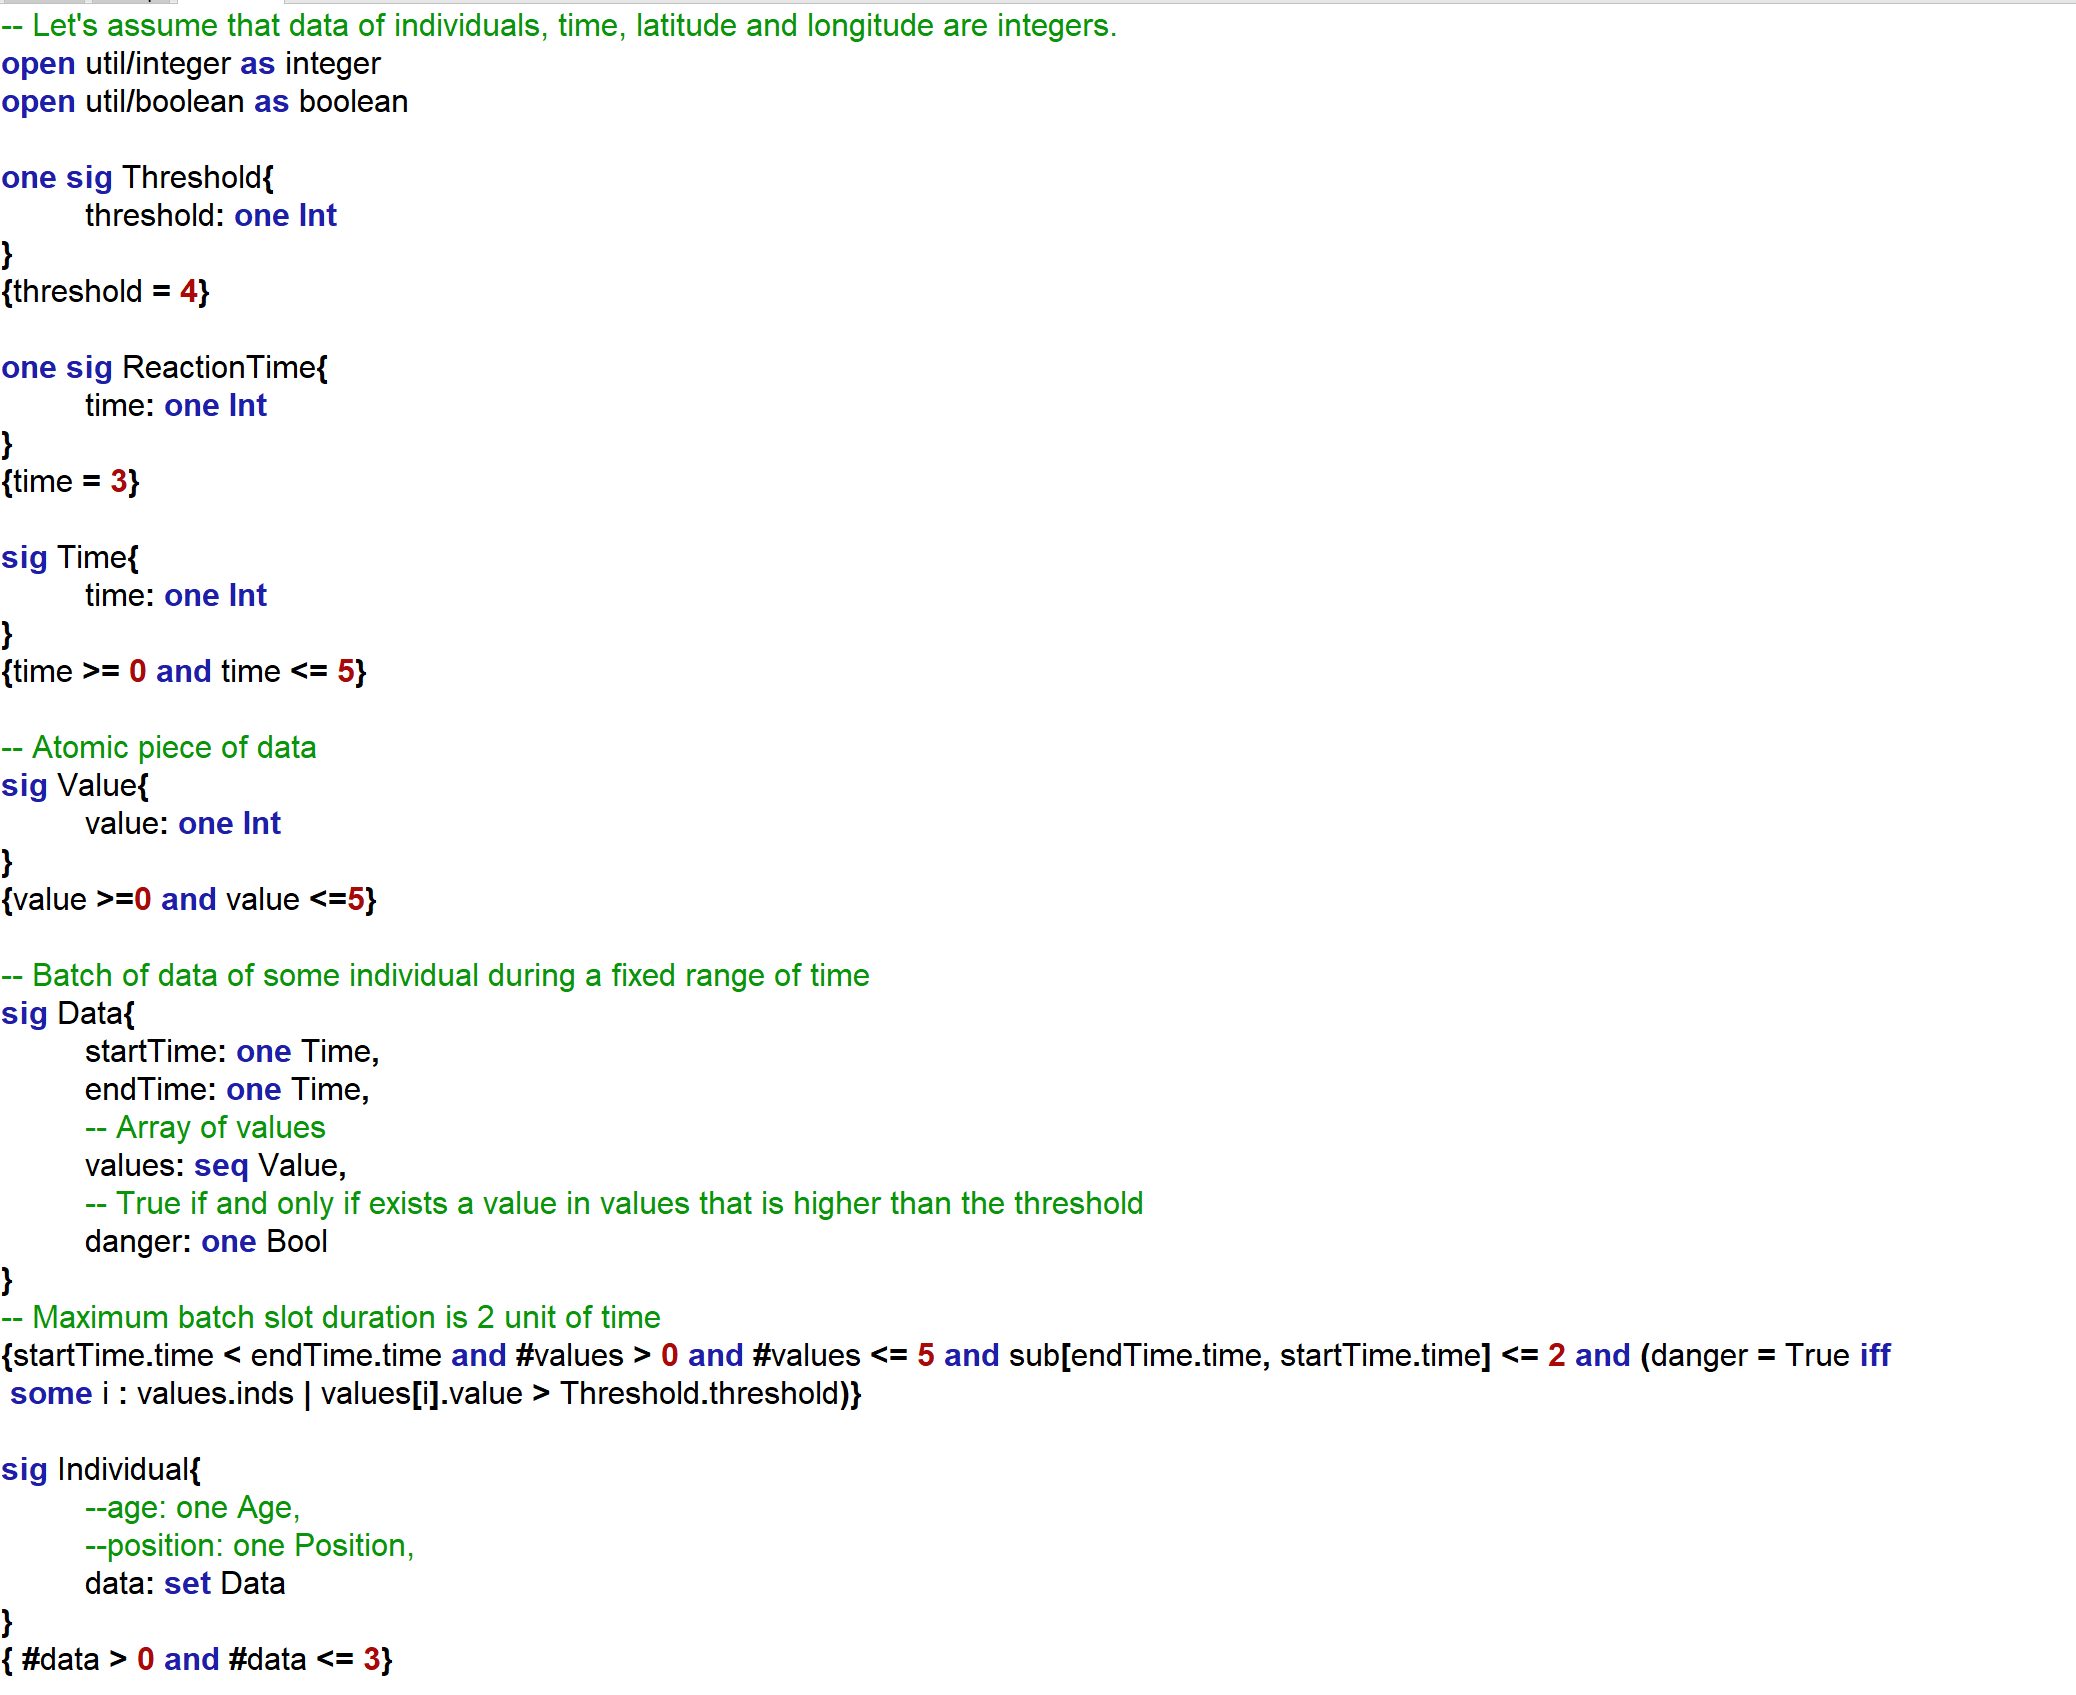
\includegraphics[width=\linewidth]{./images/alloy/code/automated_1.PNG}
		\end{figure}
		\begin{figure}[H]
			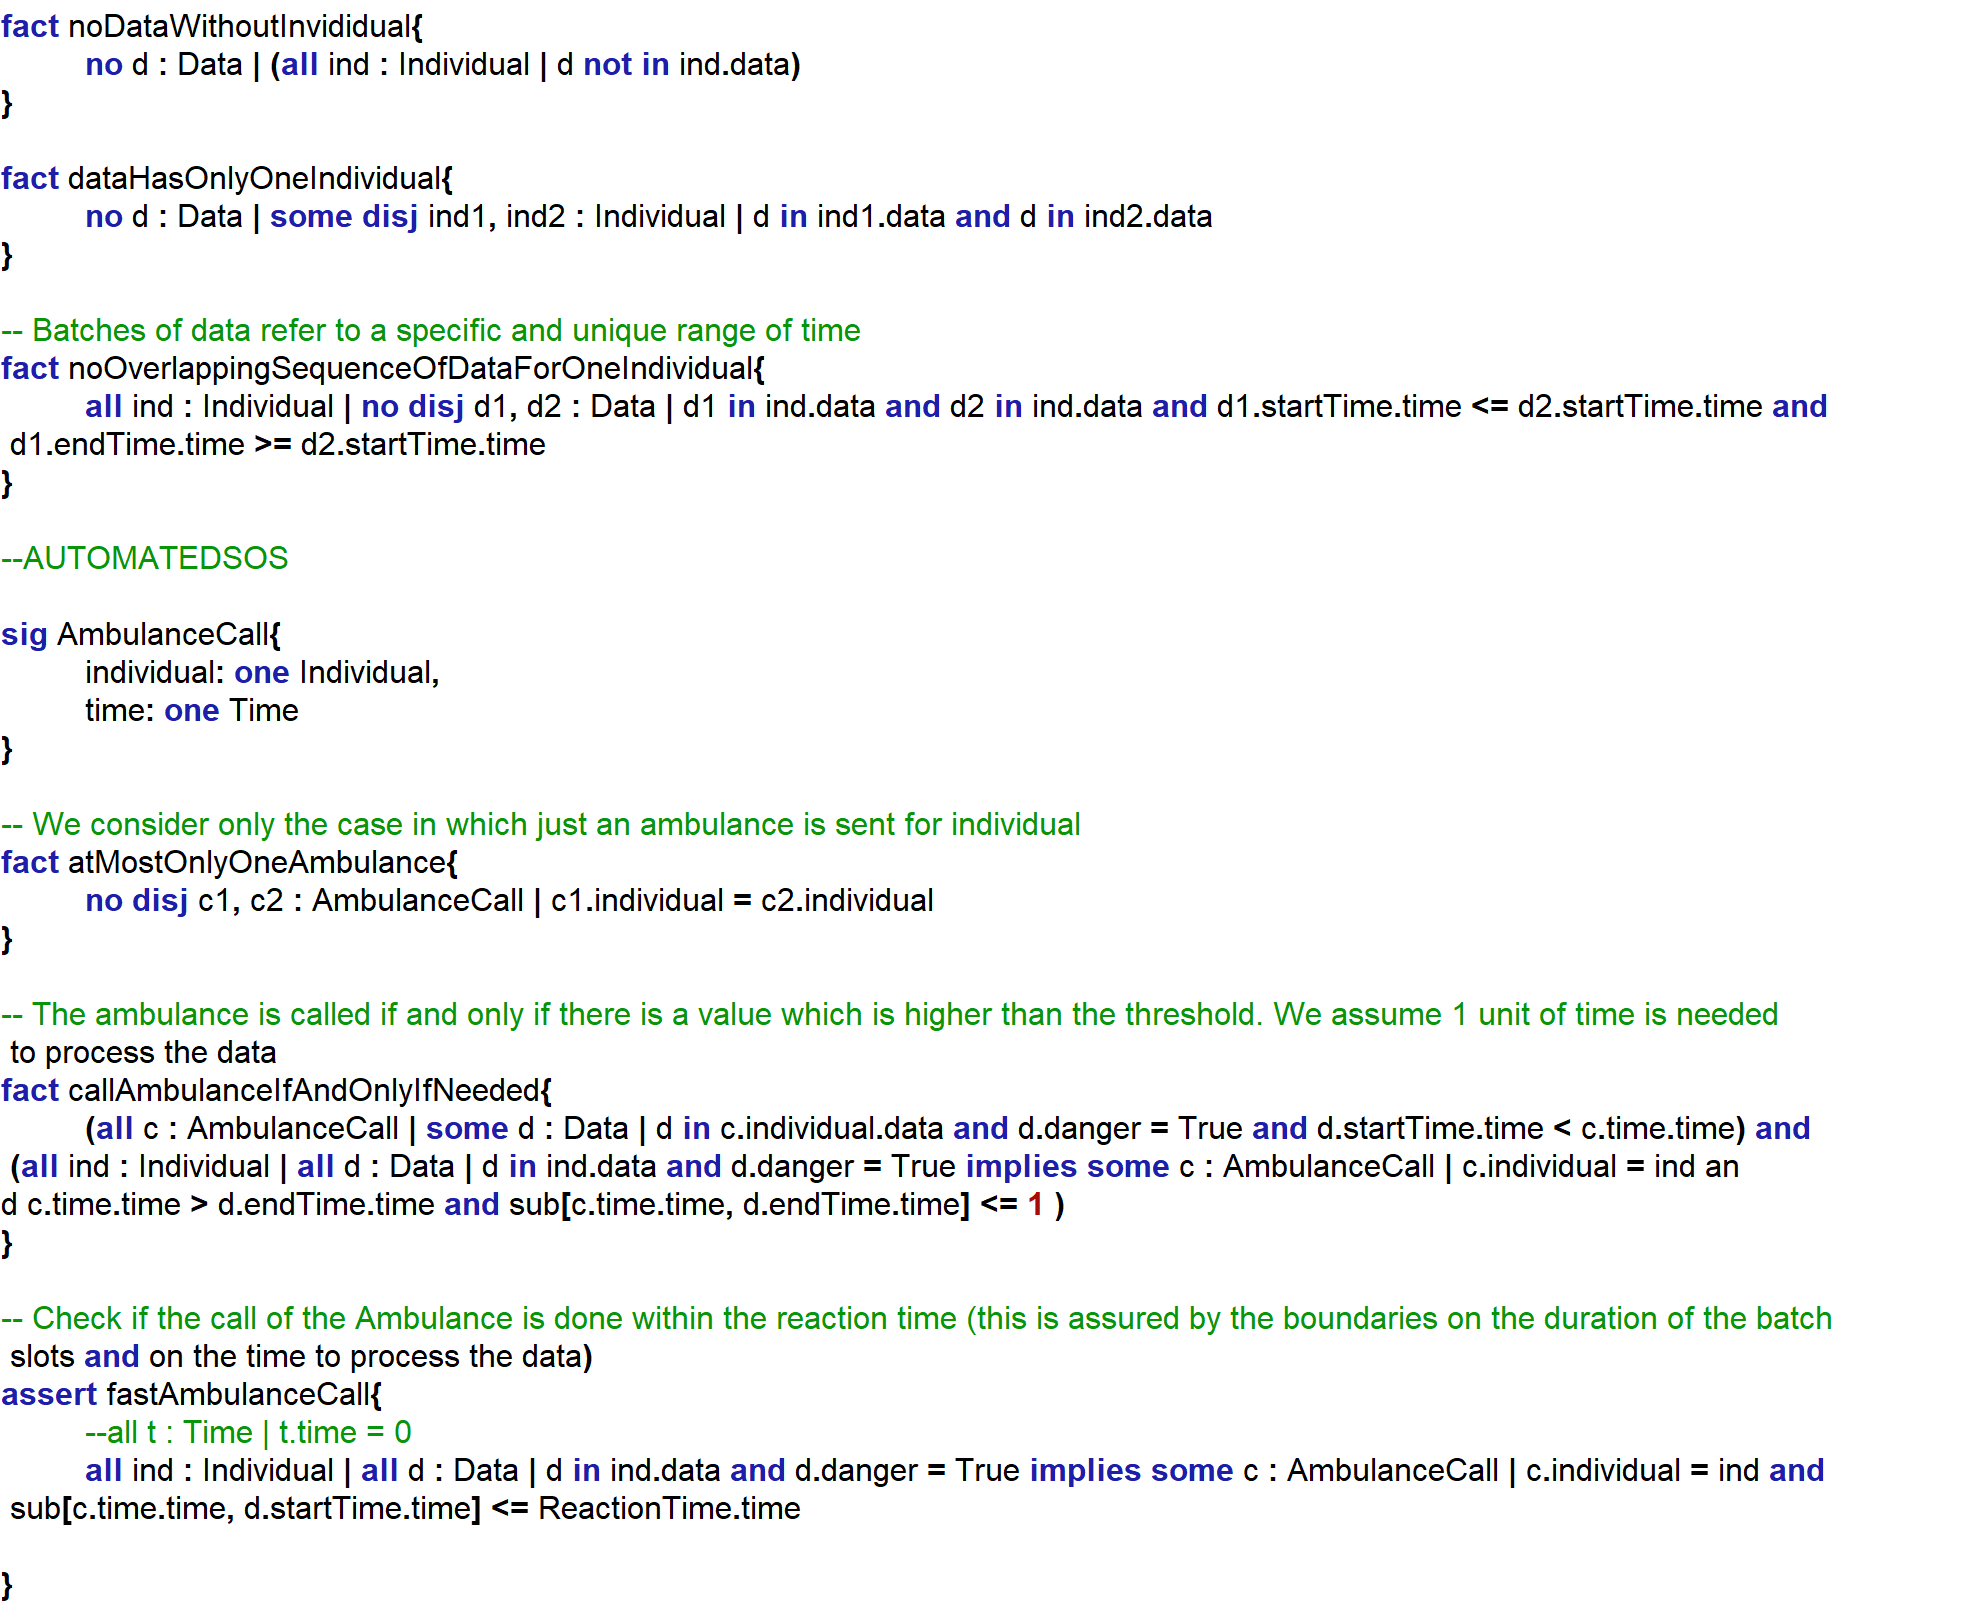
\includegraphics[width=\linewidth]{./images/alloy/code/automated_2.PNG}
			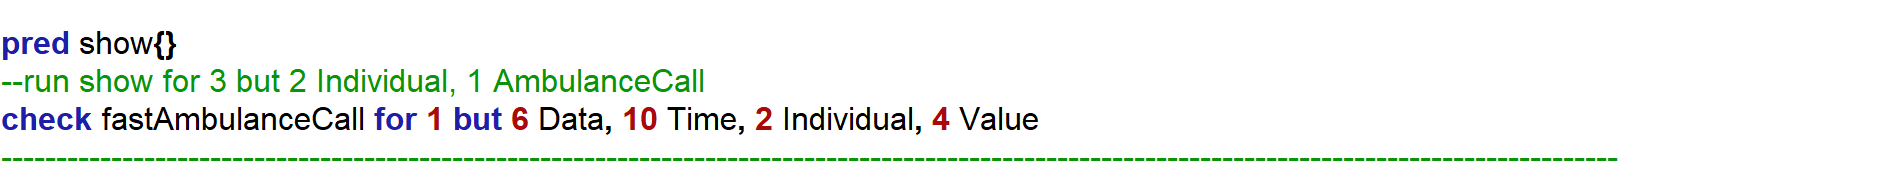
\includegraphics[width=\linewidth]{./images/alloy/code/automated_3.PNG}
		\end{figure}
		\begin{figure}[H]
			\newpage
			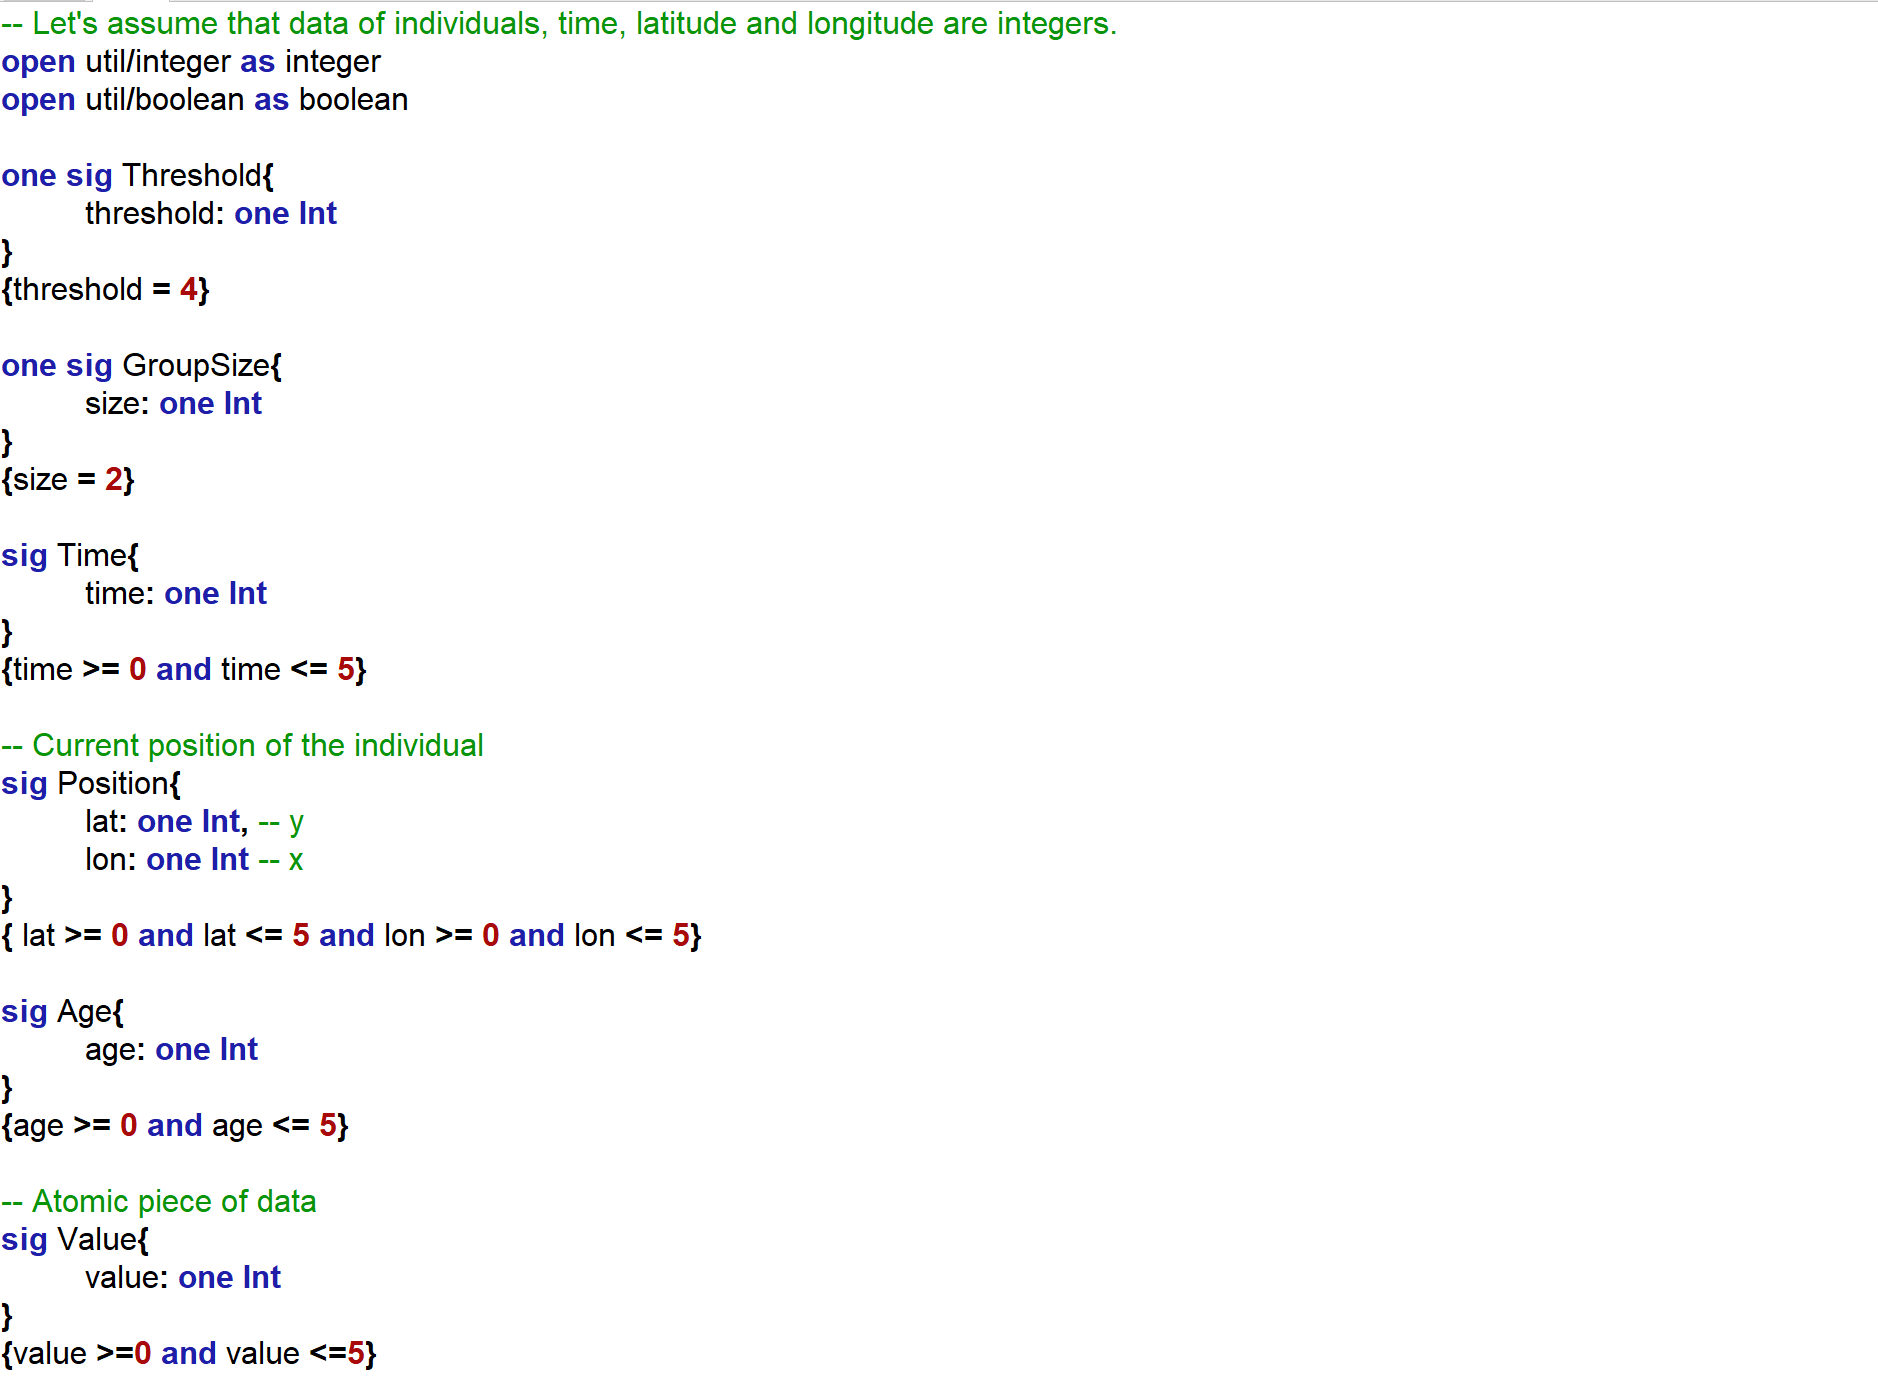
\includegraphics[width=\linewidth]{./images/alloy/code/data4Help_1.PNG}
			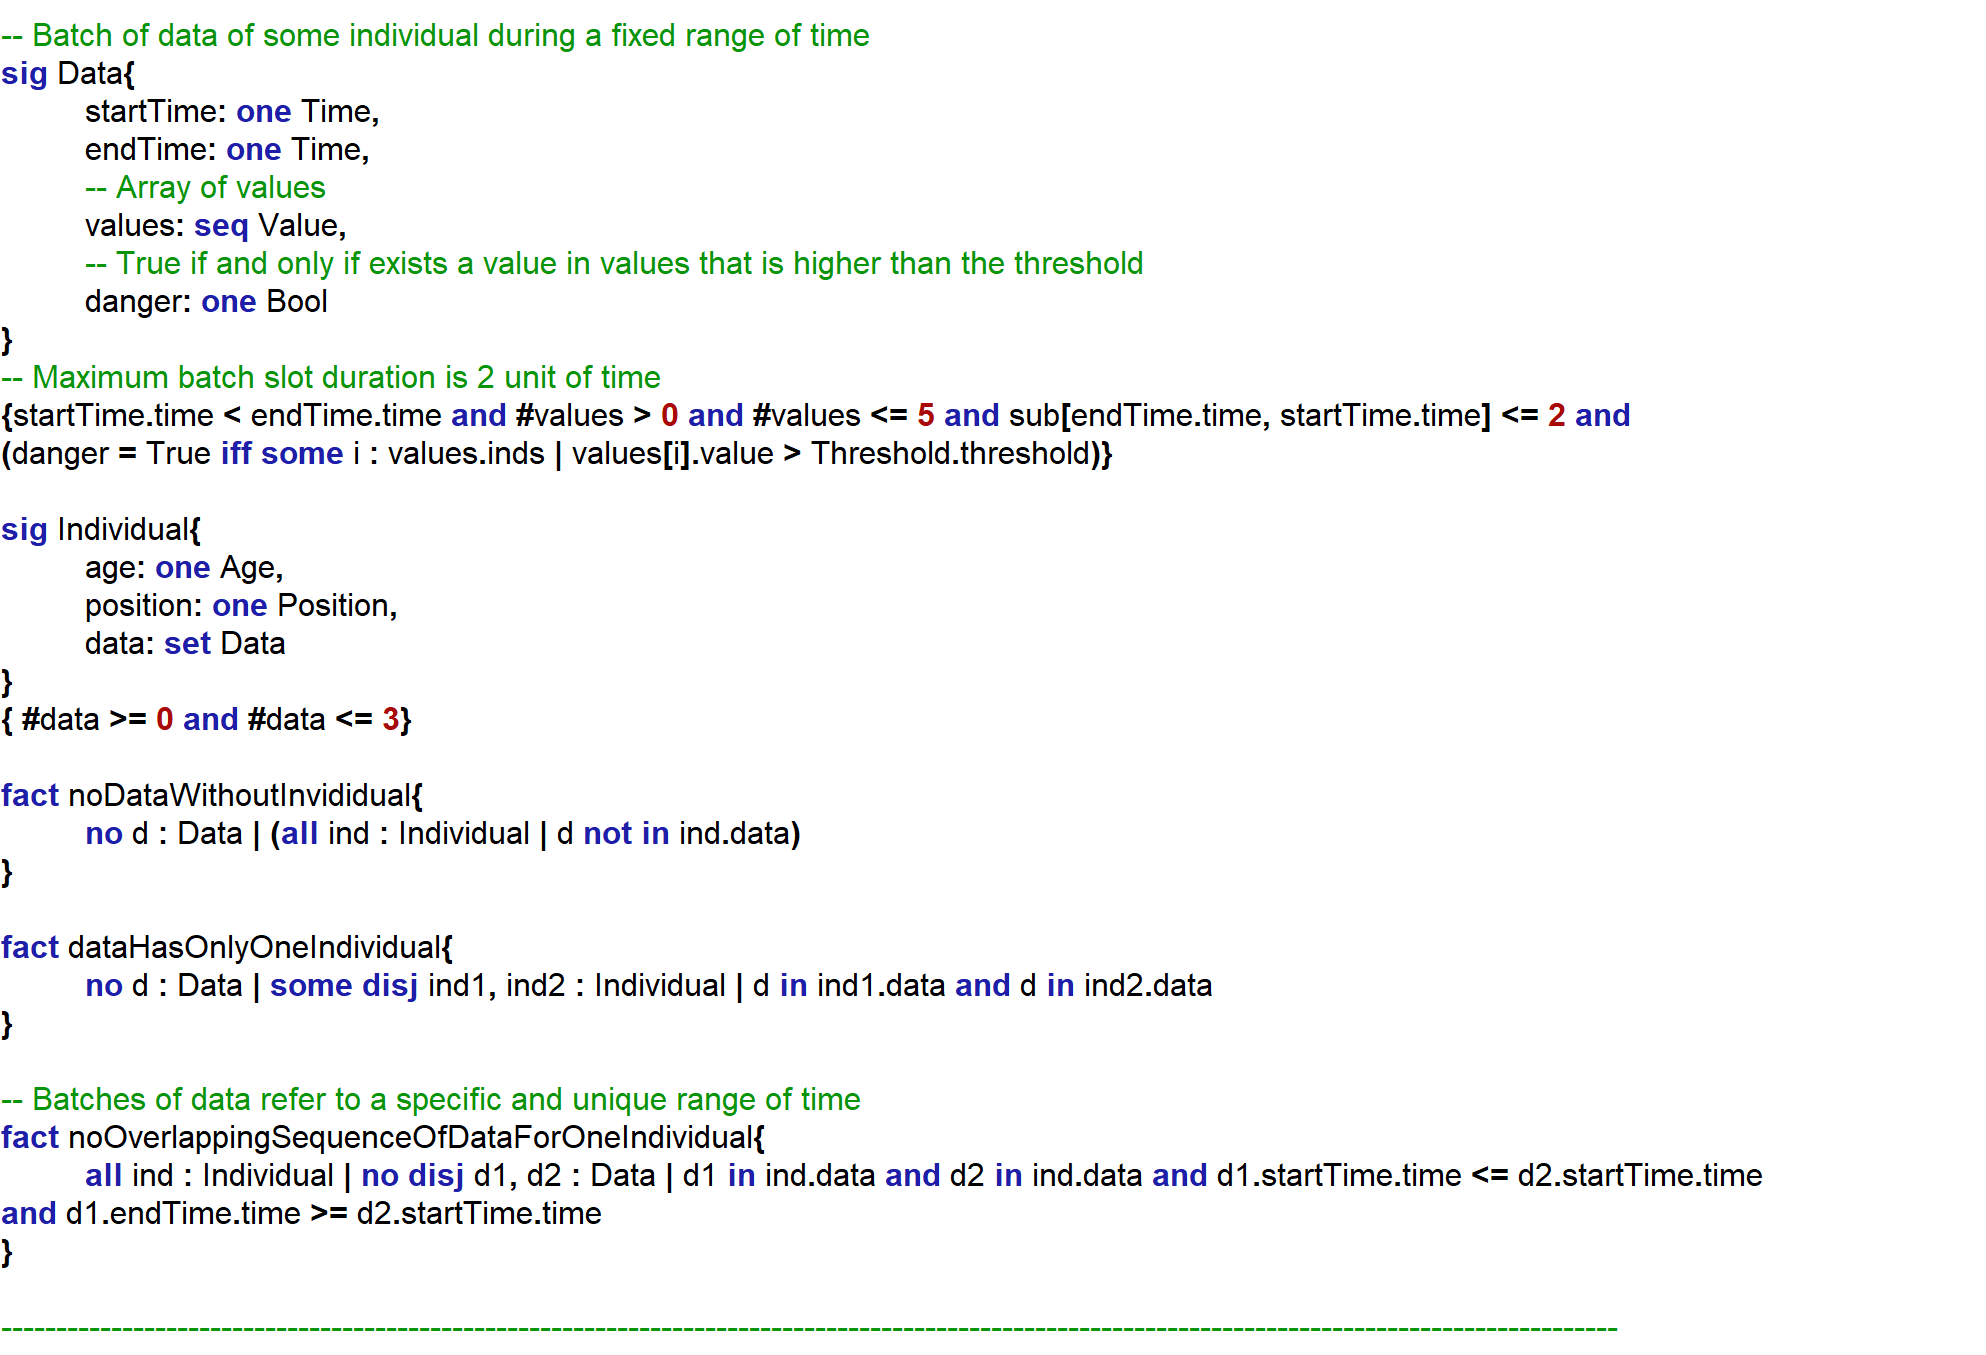
\includegraphics[width=\linewidth]{./images/alloy/code/data4Help_2.PNG}
		\end{figure}
		\begin{figure}[H]
			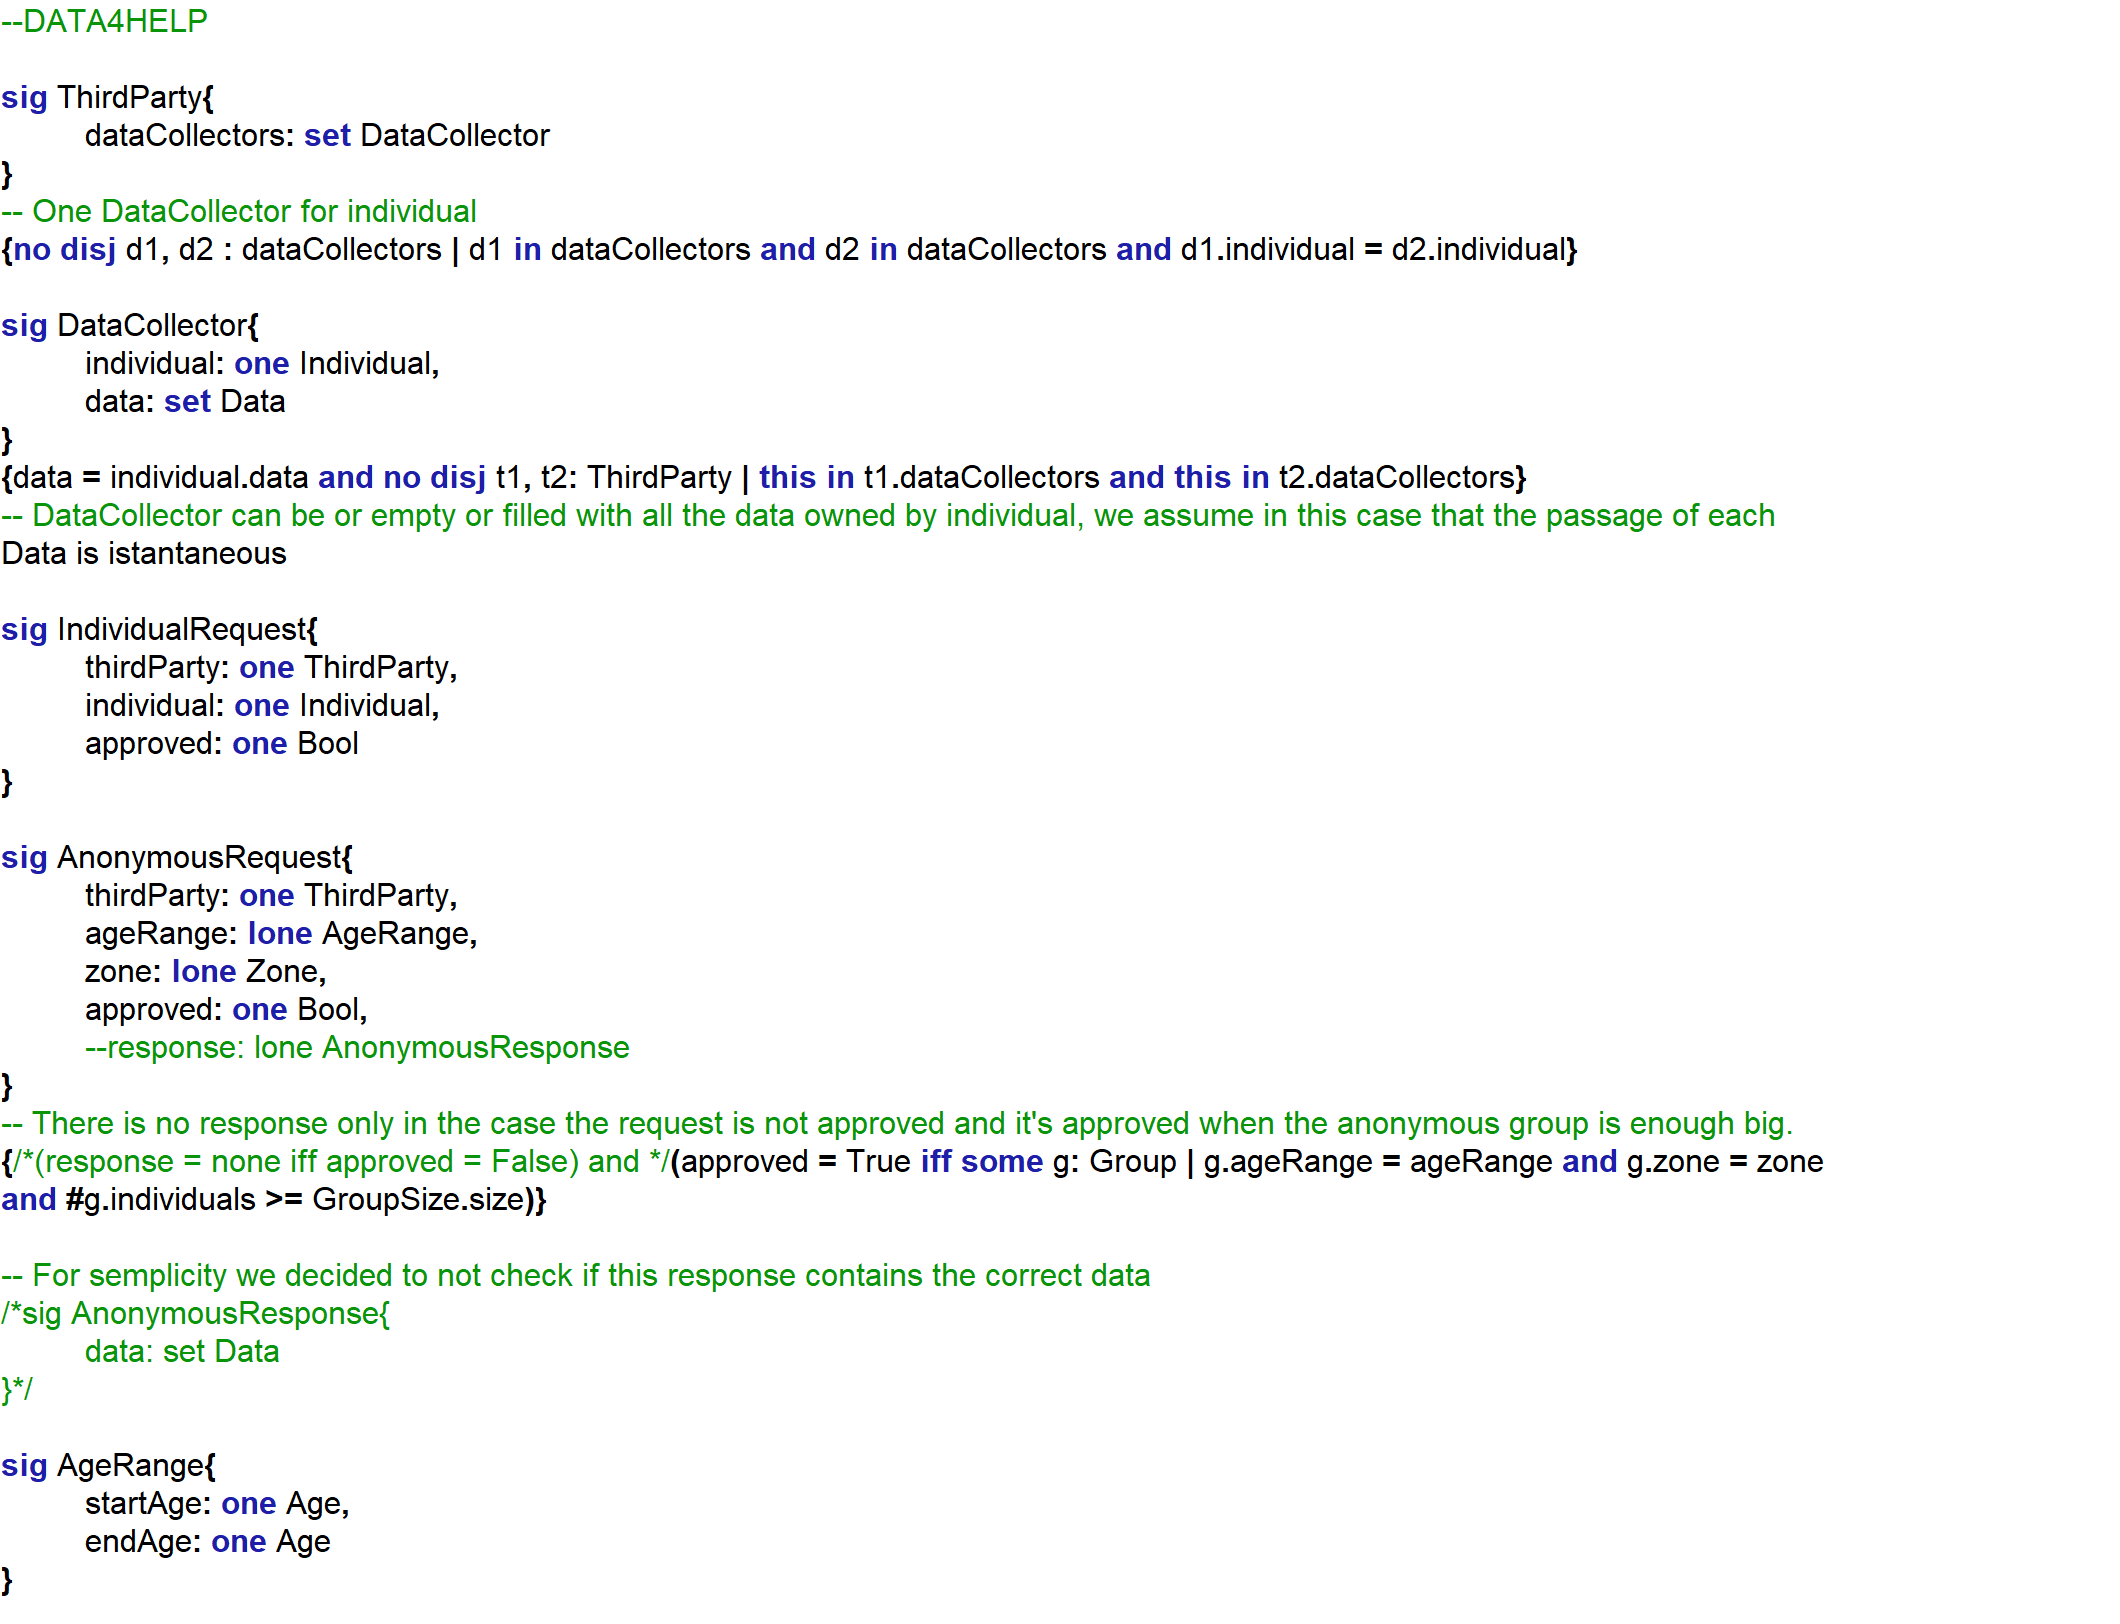
\includegraphics[width=\linewidth]{./images/alloy/code/data4Help_3.PNG}
			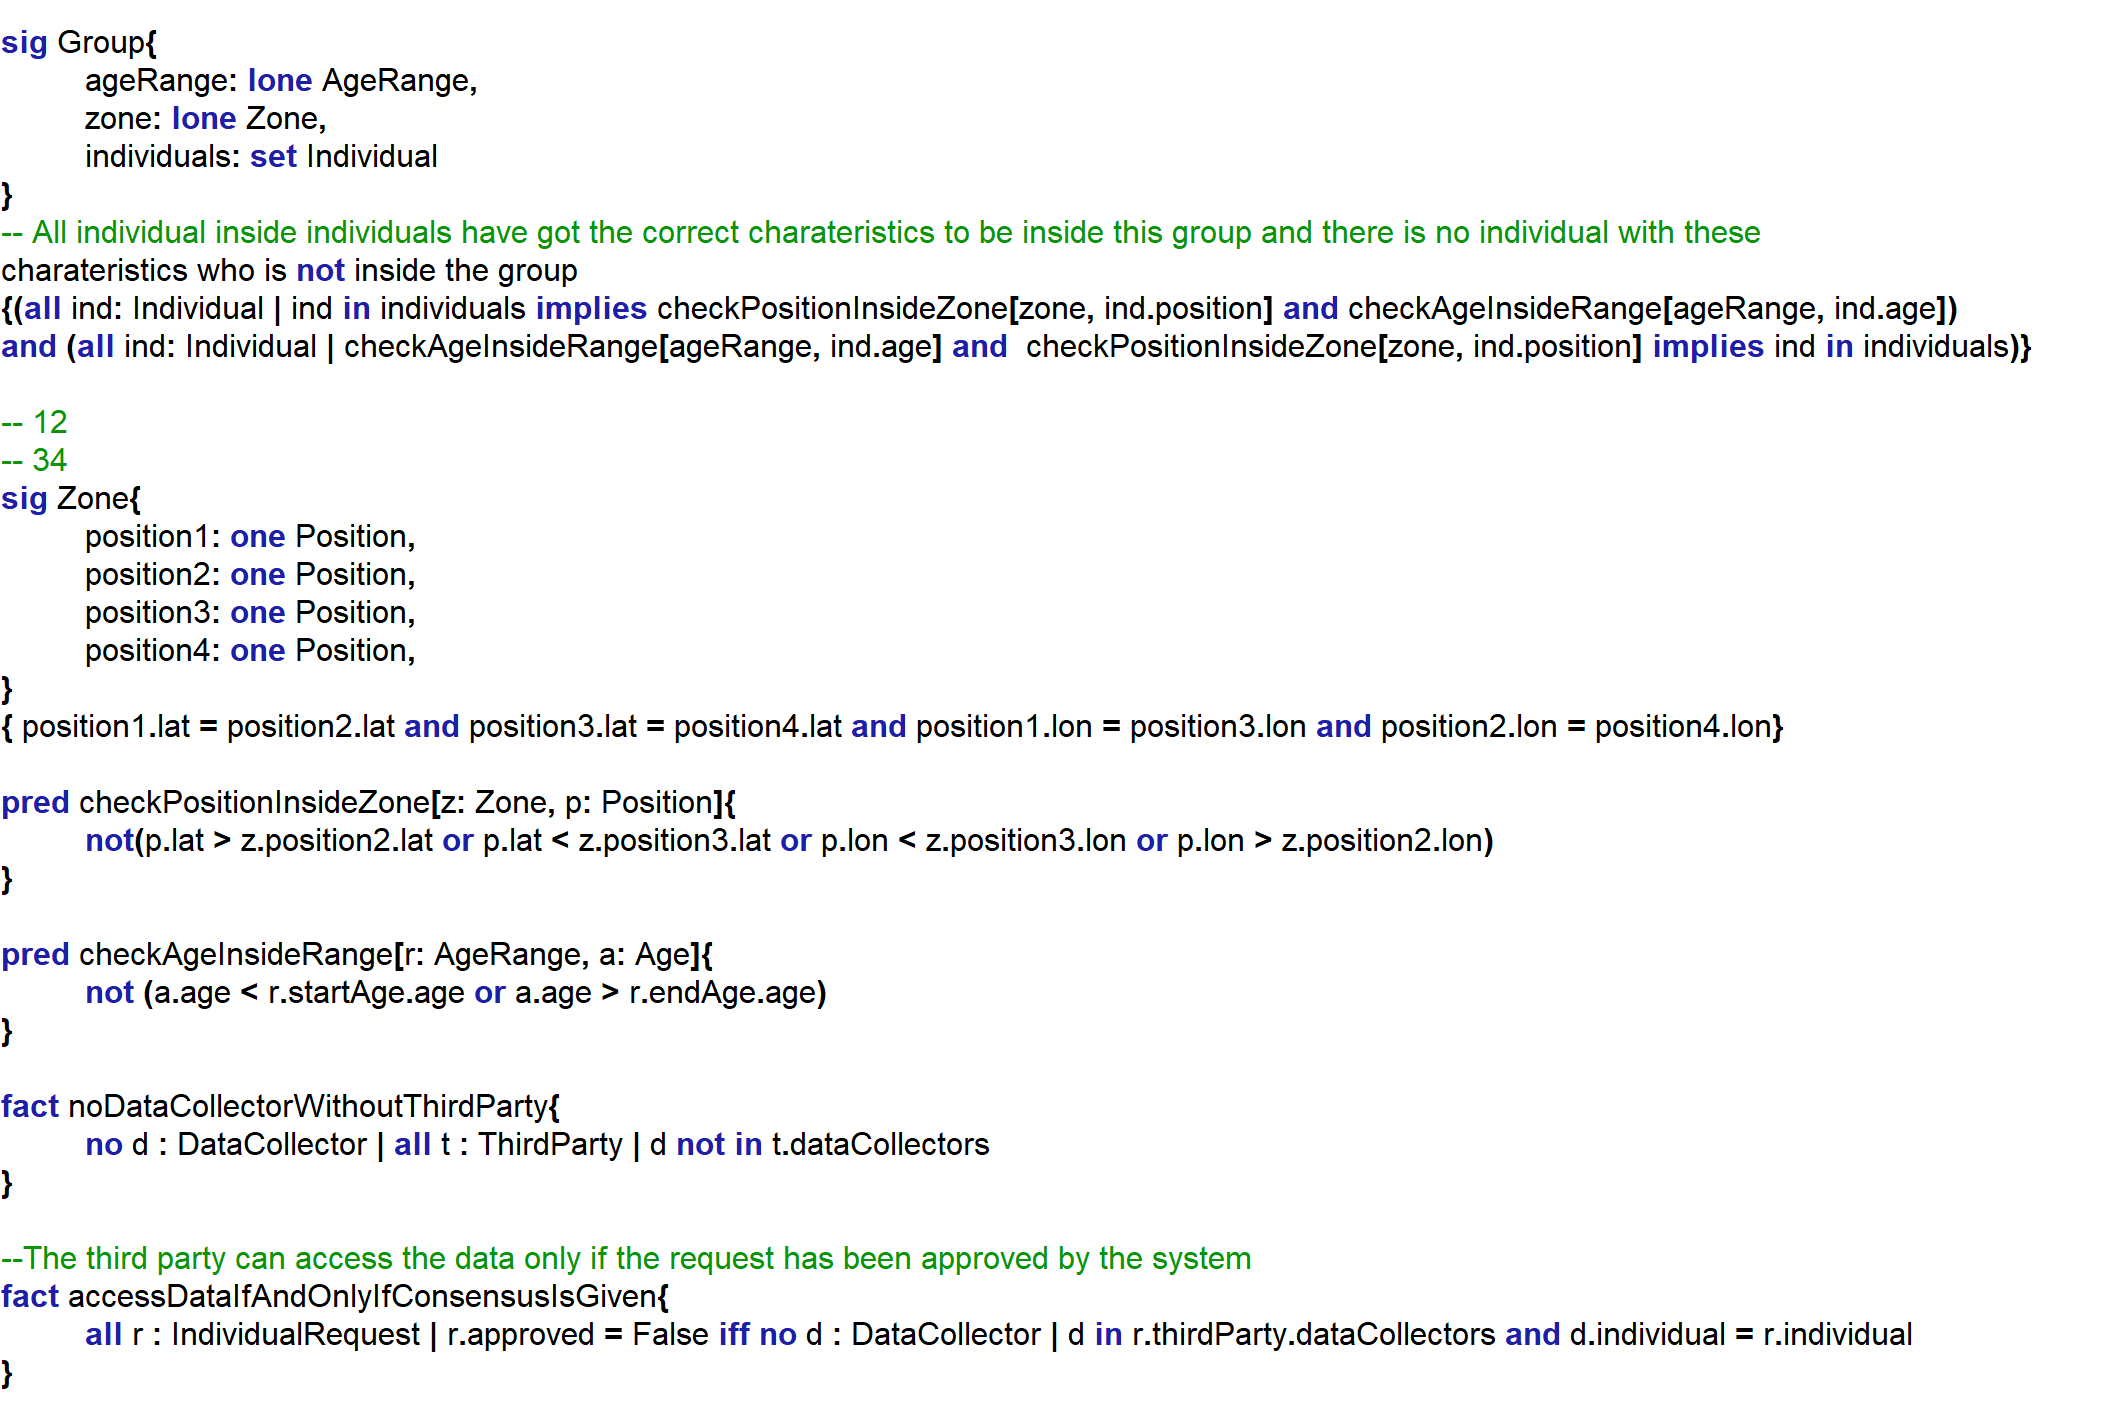
\includegraphics[width=\linewidth]{./images/alloy/code/data4Help_4.PNG}
		\end{figure}
		\begin{figure}[H]
			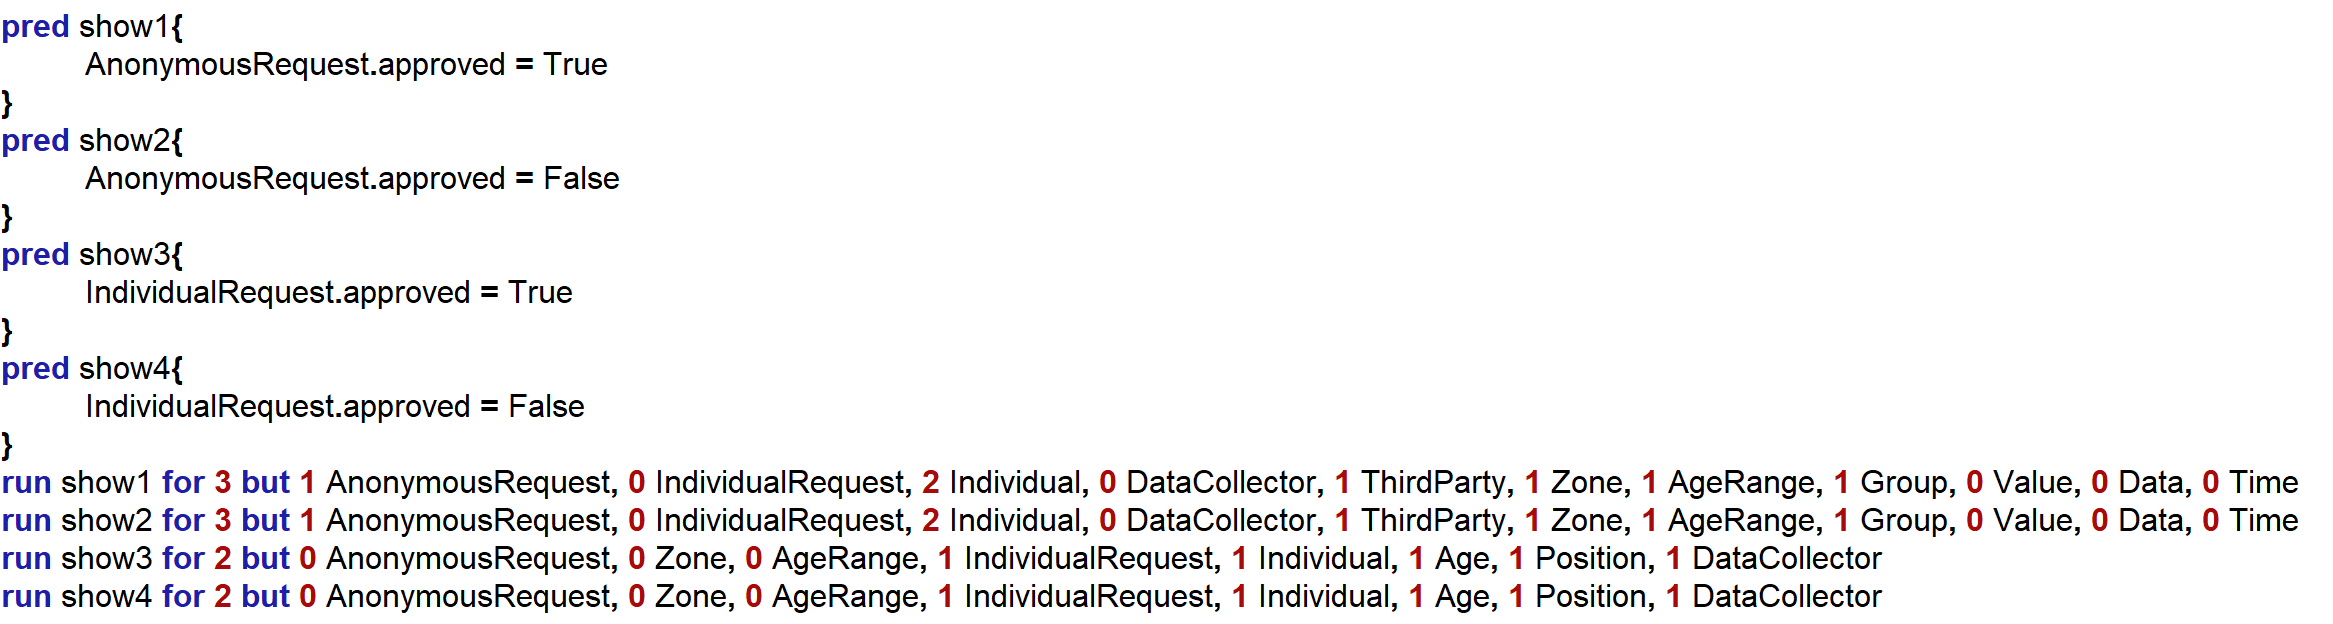
\includegraphics[width=\linewidth]{./images/alloy/code/data4Help_5.PNG}
		\end{figure}
		\newpage
		\begin{figure}[H]
			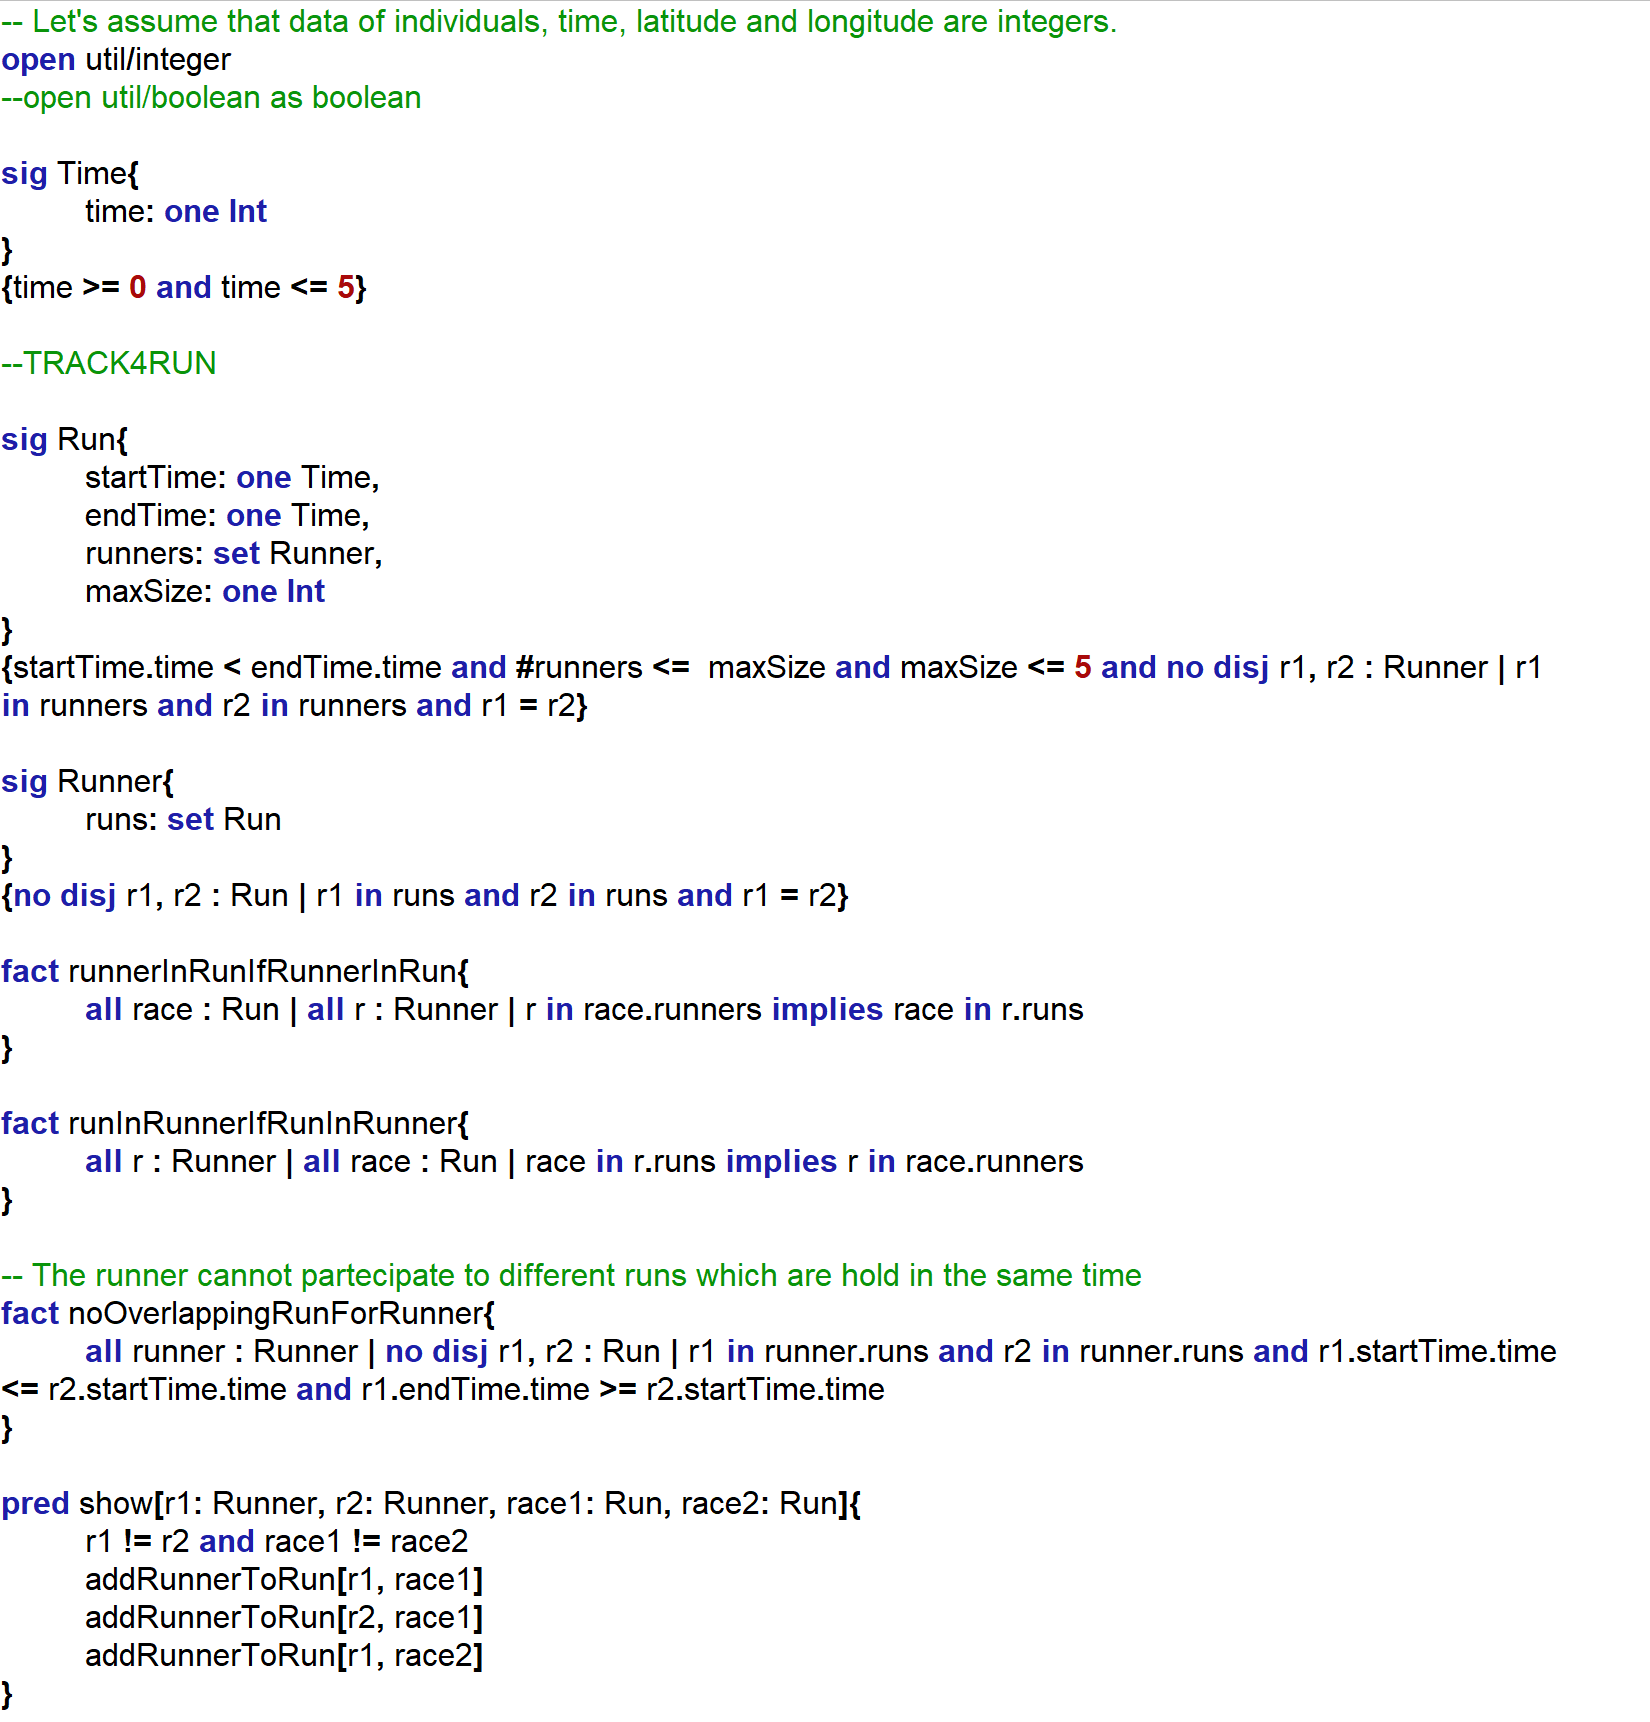
\includegraphics[width=\linewidth]{./images/alloy/code/track4Run_1.PNG}
		\end{figure}
		\begin{figure}[H]
			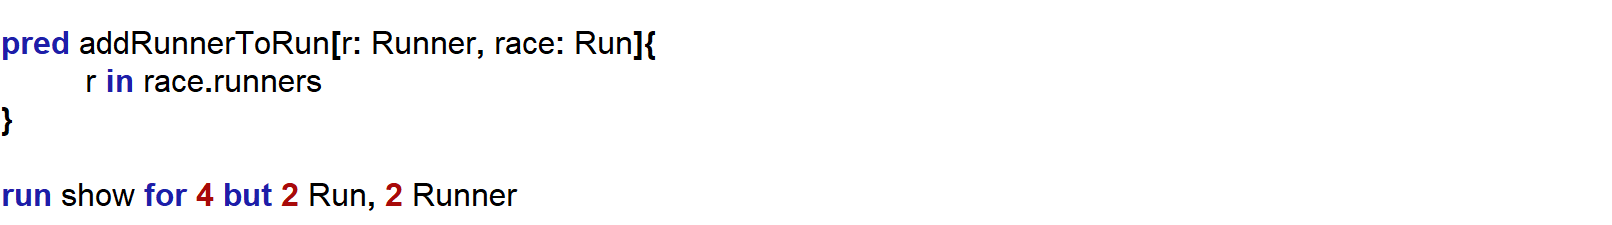
\includegraphics[width=\linewidth]{./images/alloy/code/track4Run_2.PNG}
		\end{figure}		
		\begin{itemize}
			\newpage
			\item Anonymous request accepted
			\begin{figure}[H]
		  				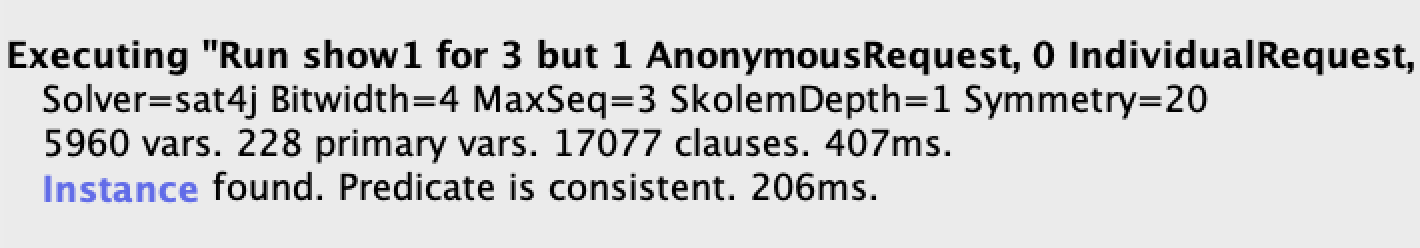
\includegraphics[width=\linewidth]{./images/alloy/anonymous-request-true-Run.png}
		  				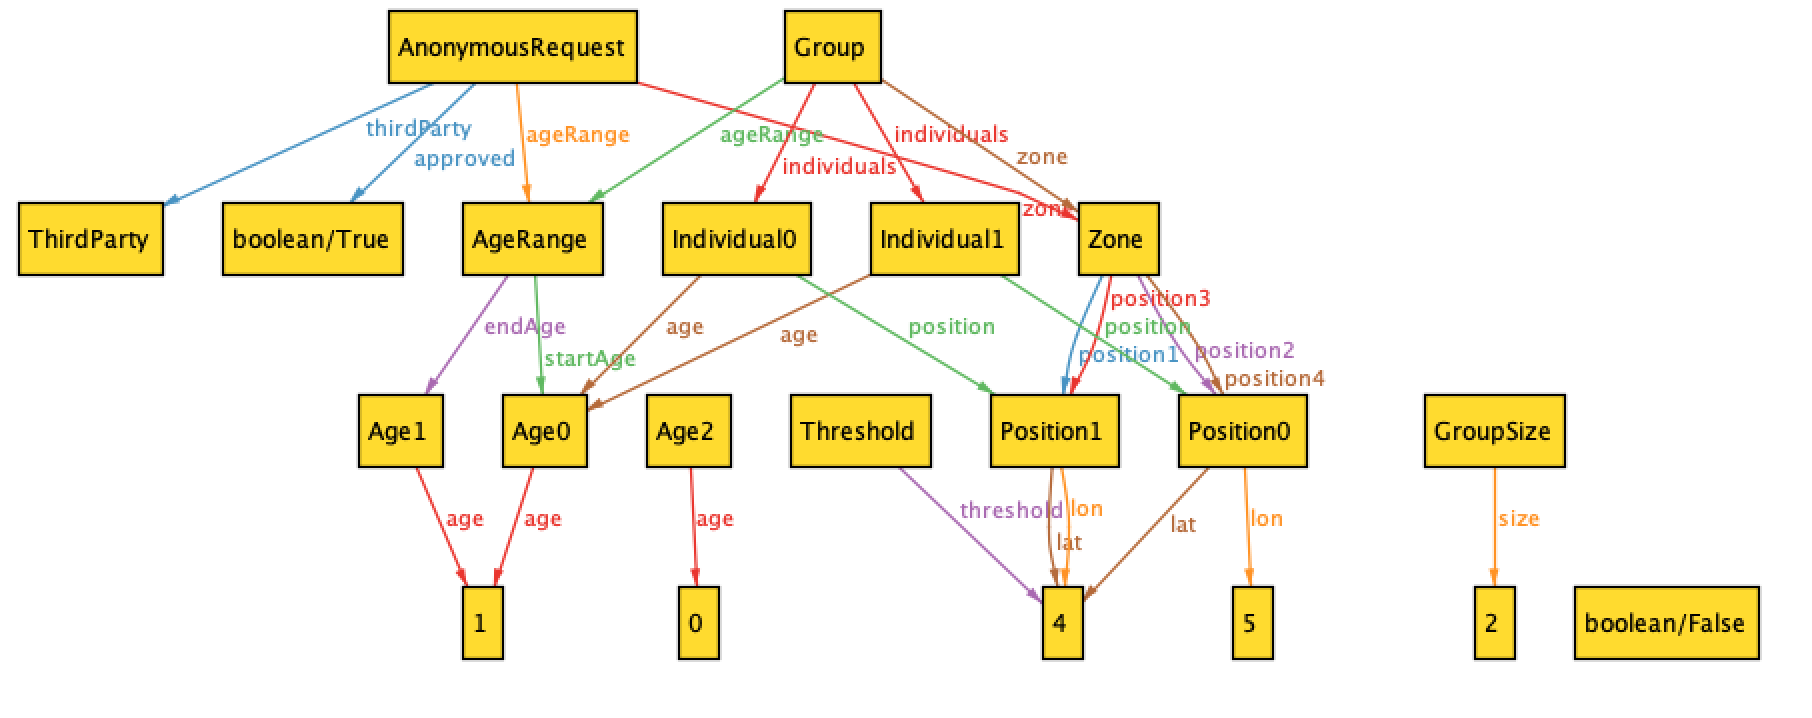
\includegraphics[width=\linewidth]{./images/alloy/anonymous-request-true-World.png}
			\end{figure}
			\item Anonymous request refused
			\begin{figure}[H]
		  				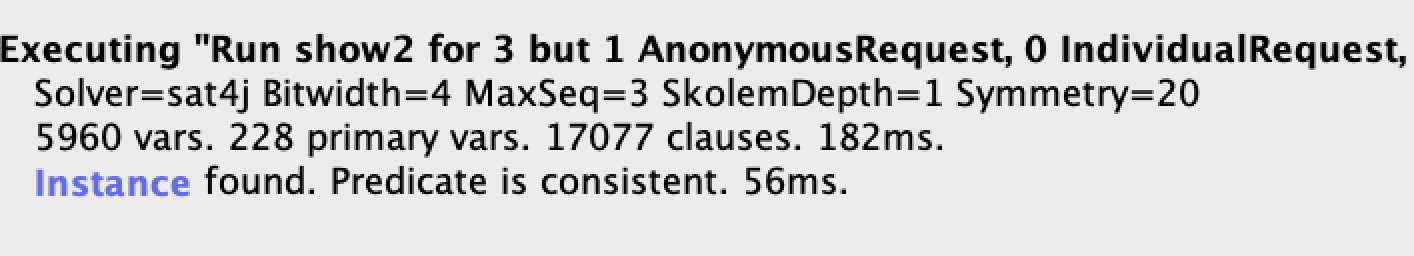
\includegraphics[width=\linewidth]{./images/alloy/anonymous-request-false-Run.png}
		  				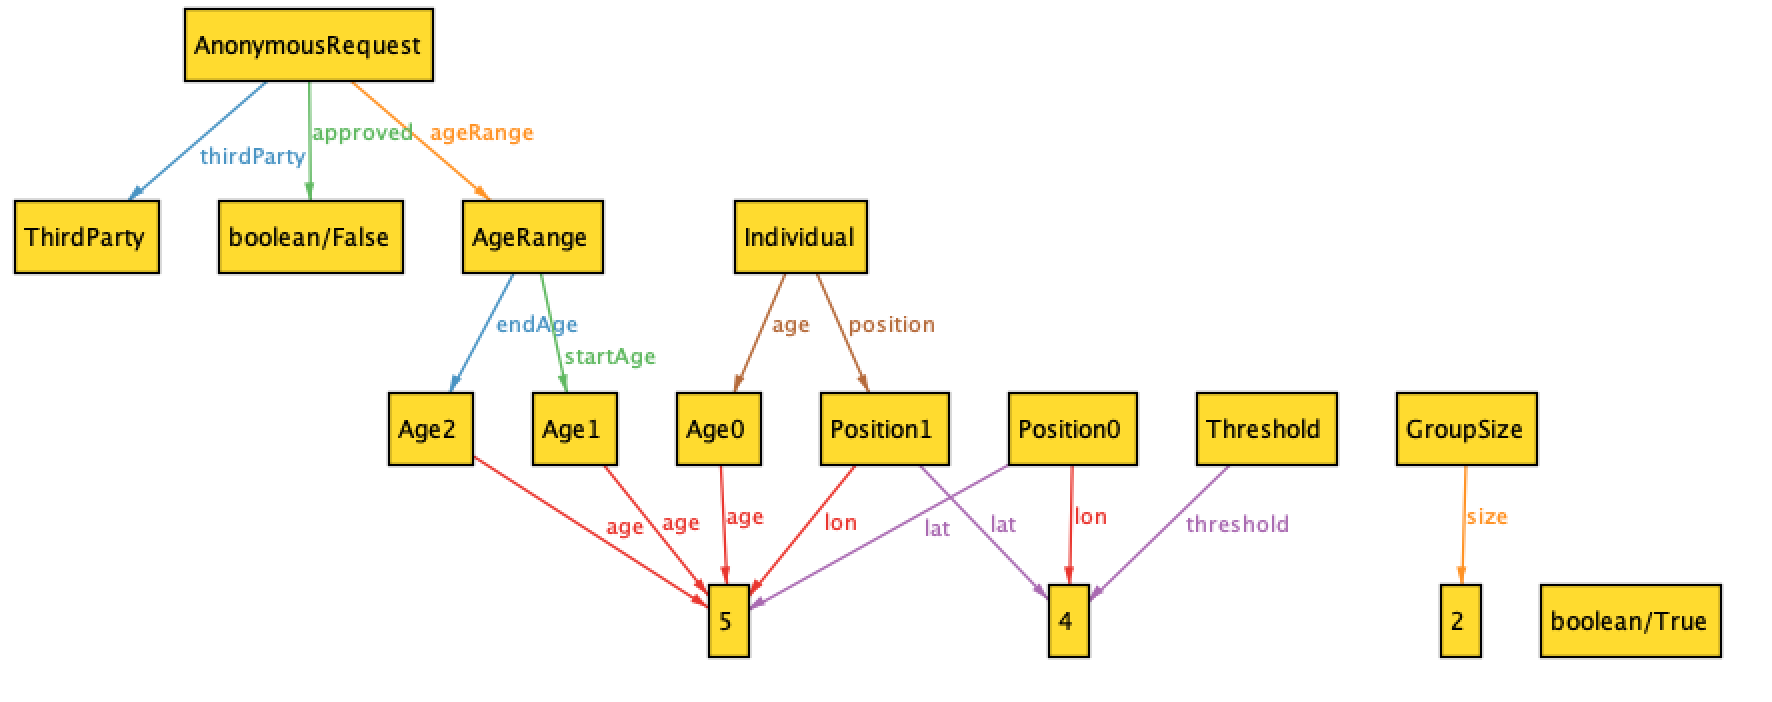
\includegraphics[width=\linewidth]{./images/alloy/anonymous-request-false-World.png}
			\end{figure}
			\newpage
			\item Individual request accepted
			\begin{figure}[H]
		  				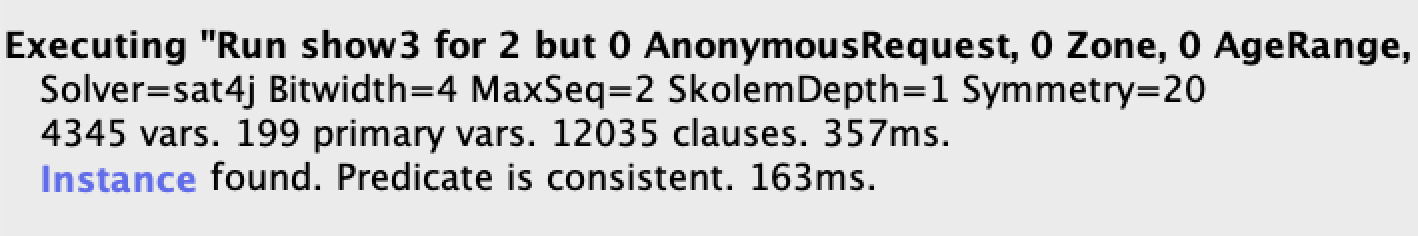
\includegraphics[width=\linewidth]{./images/alloy/individual-request-true-Run.png}
		  				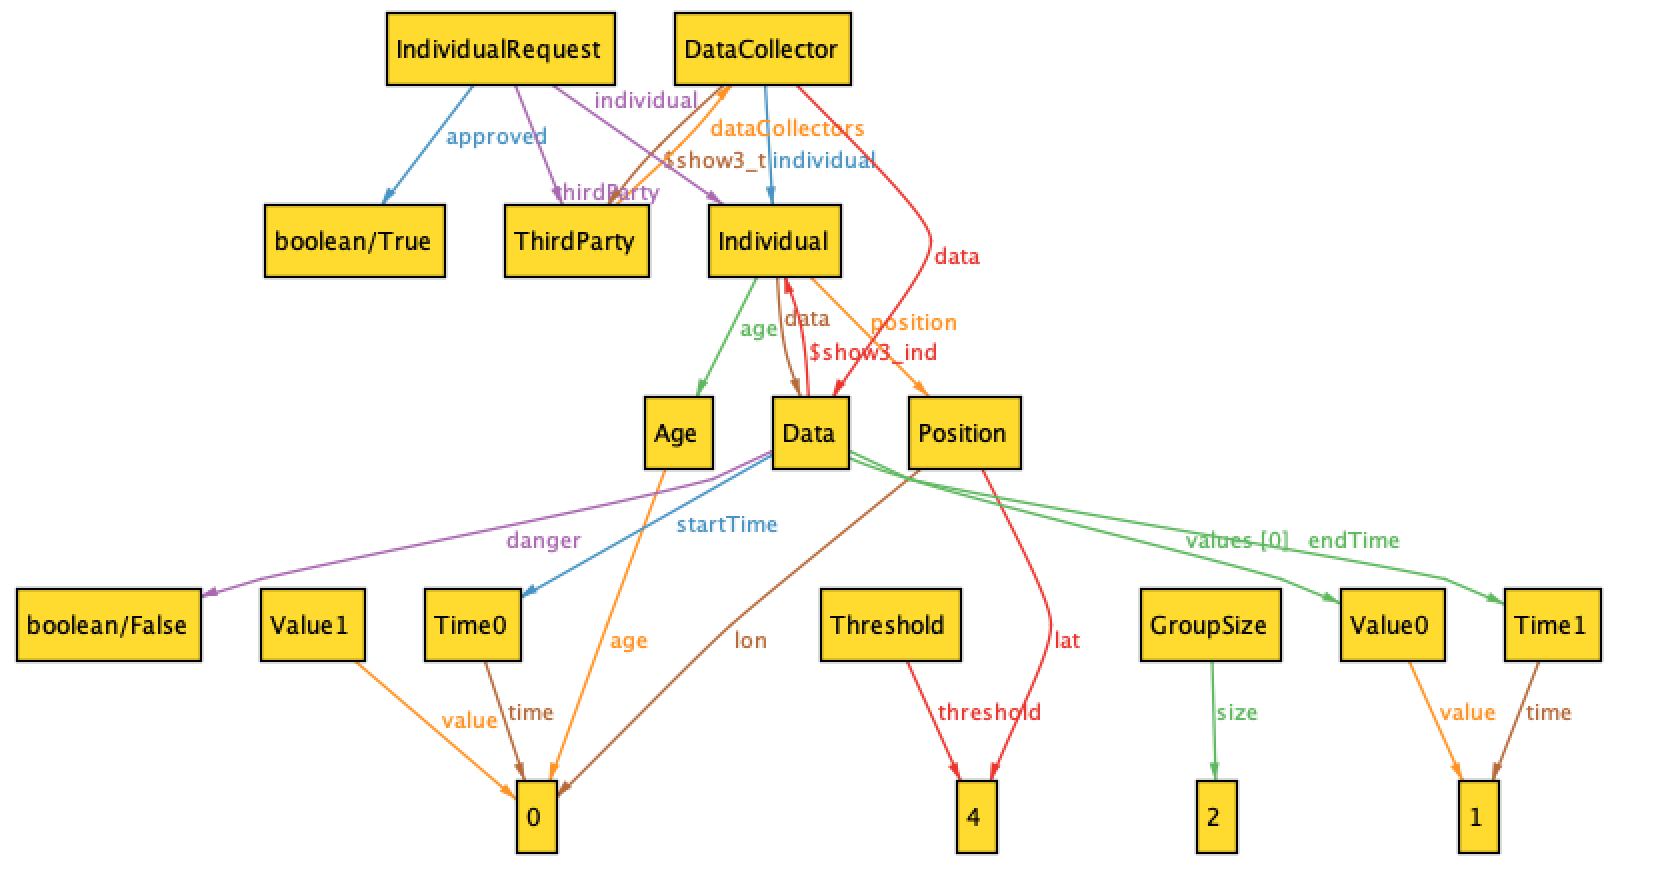
\includegraphics[width=\linewidth]{./images/alloy/individual-request-true-World.png}
			\end{figure}
			\newpage
			\item Individual request refused
			\begin{figure}[H]
		  				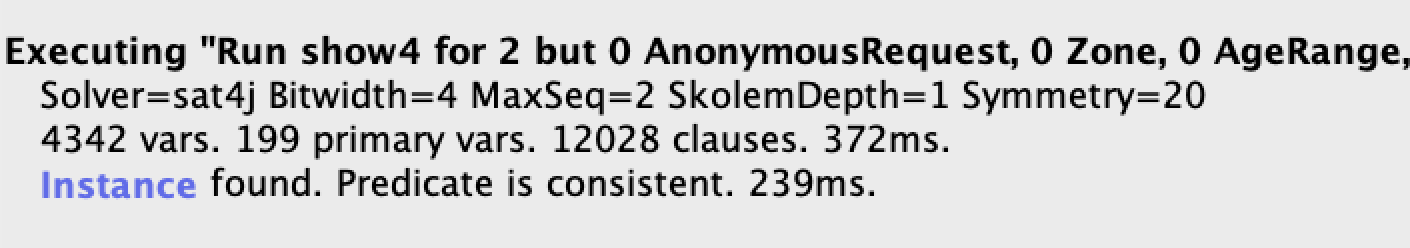
\includegraphics[width=\linewidth]{./images/alloy/individual-request-false-Run.png}
		  				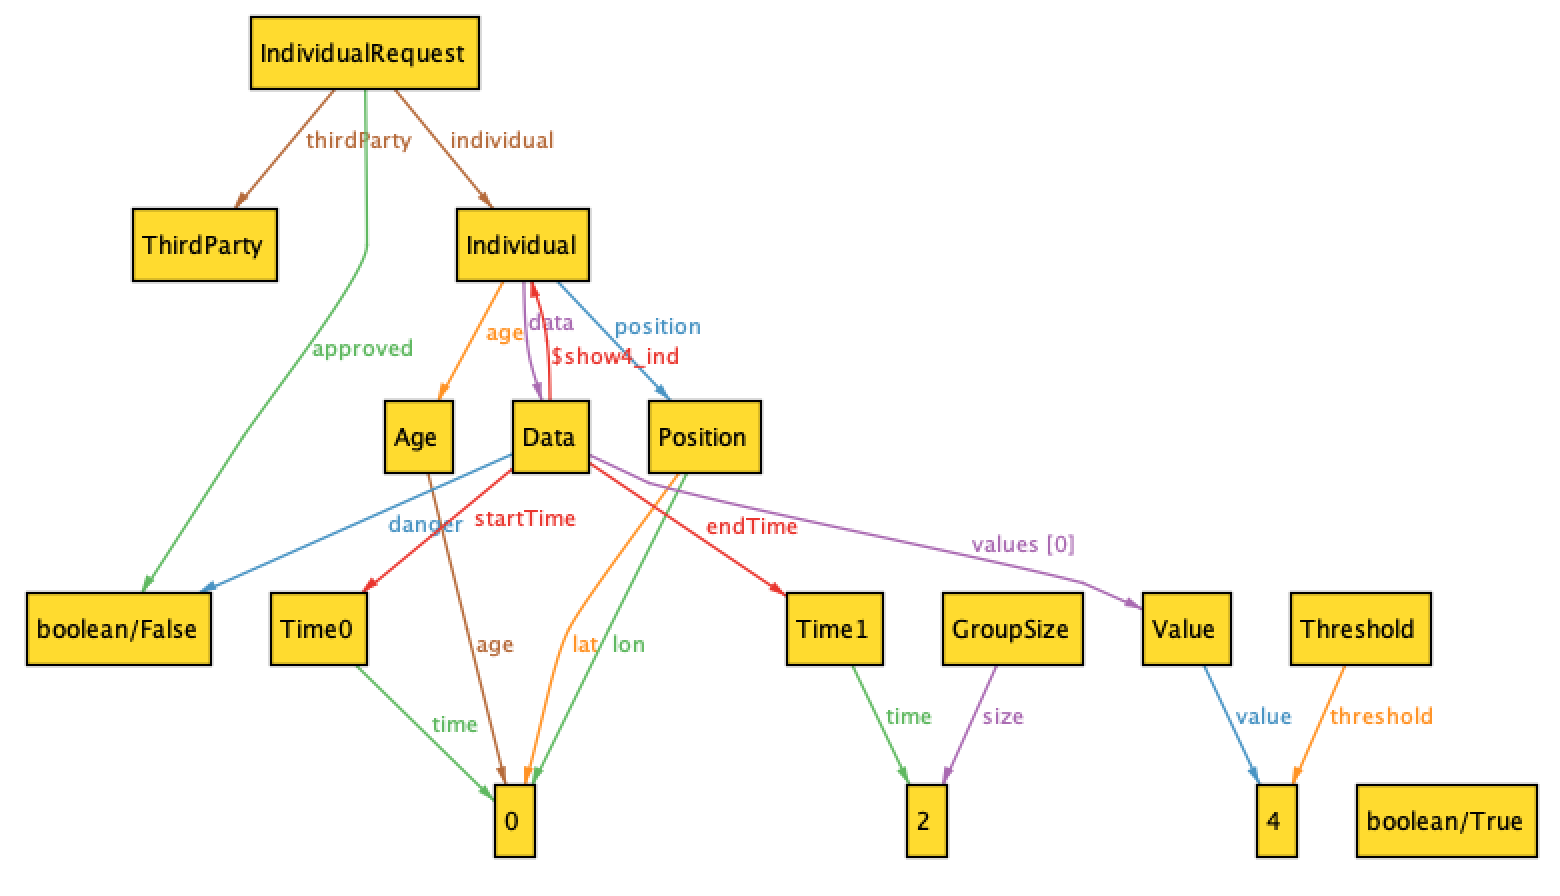
\includegraphics[width=\linewidth]{./images/alloy/individual-request-false-World.png}
			\end{figure}
			\newpage
			\item Check assertion on AutomatedSOS
			\begin{figure}[H]
		  				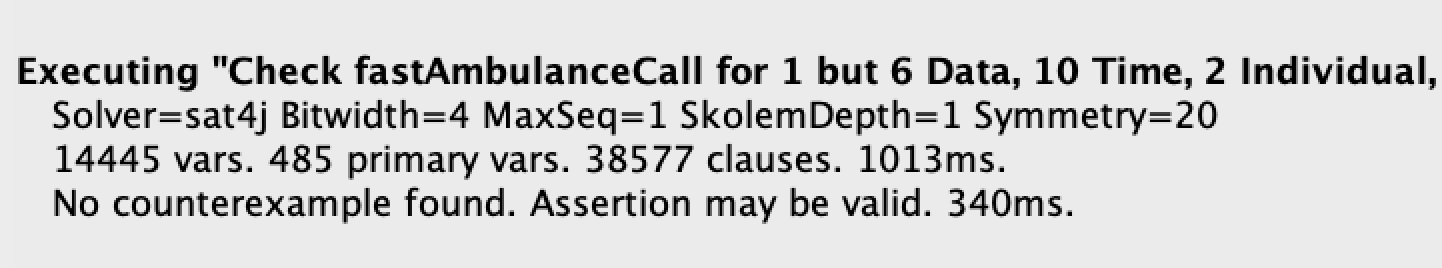
\includegraphics[width=\linewidth]{./images/alloy/automatedSOS-Assert.png}
			\end{figure}
			\item Ambulance call
			\begin{figure}[H]
		  				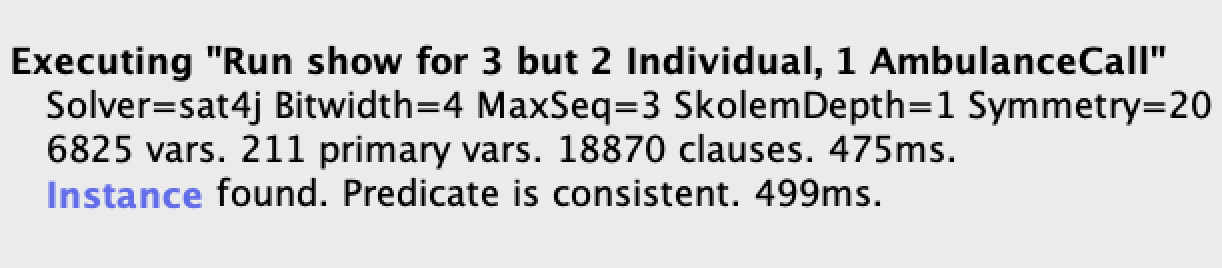
\includegraphics[width=\linewidth]{./images/alloy/automatedSOS-Run.png}
		  				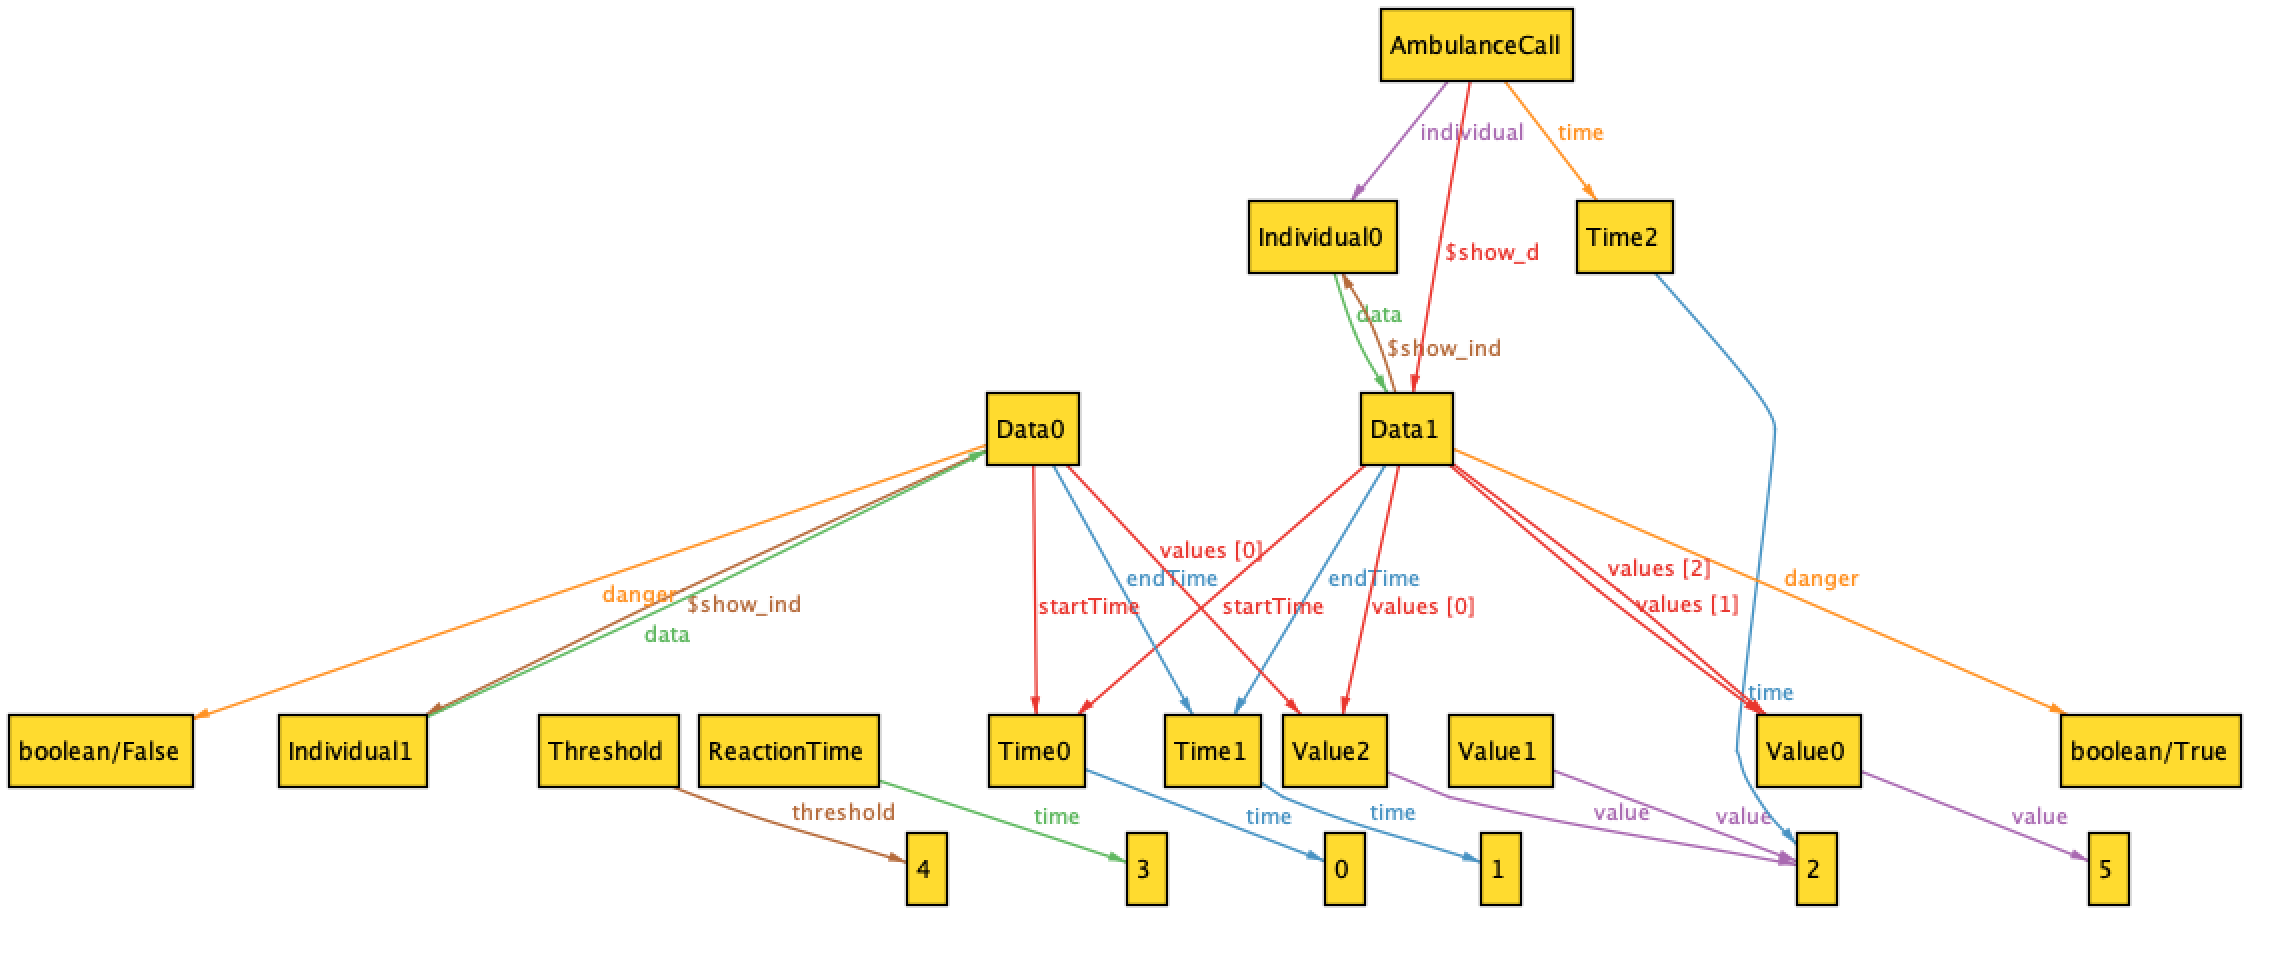
\includegraphics[width=\linewidth]{./images/alloy/automatedSOS-World.png}
			\end{figure}
			\newpage
			\item Track4Run
			\begin{figure}[H]
		  				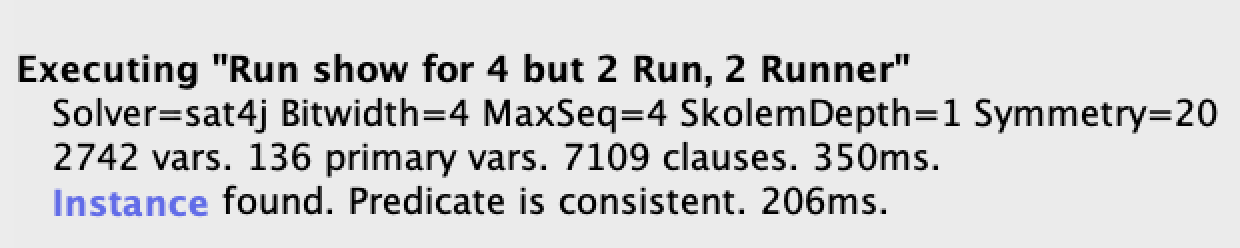
\includegraphics[width=\linewidth]{./images/alloy/track4Run-Run.png}
		  				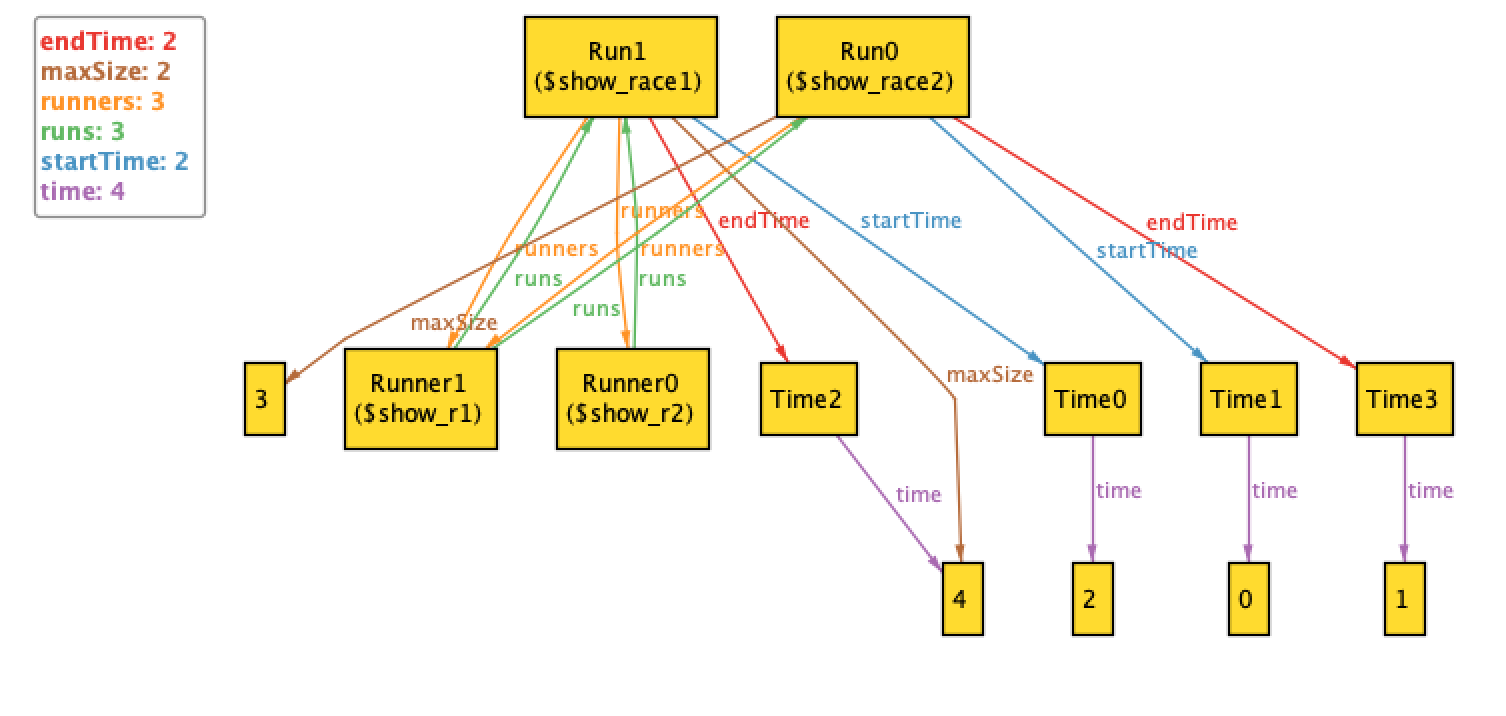
\includegraphics[width=\linewidth]{./images/alloy/track4Run-World.png}
			\end{figure}
		\end{itemize}
	\newpage
	\item \underline{Effort spent}\\
		{\normalfont
		\begin{itemize}
		\item \textbf{Paolo Romeo}\\\\
				%Table of effort
				\begin{tabular}{| m{9cm} | m{3cm}| }
				\hline
					\textbf{Description of the task} & \textbf{Hours spent}\\
				\hline
					Definition of goals, requirements and assumptions & 7 \\
				\hline
					Product perspective and functions & 4 \\
				\hline
					Specific requirements & 4 \\
				\hline
					Formal analysis using Alloy & 3 \\
				\hline
					Other related activities & 7 \\
				\hline
				\end{tabular}
				\\\\\\
		\item \textbf{Andrea Scotti}\\\\
				%Table of effort
				\begin{tabular}{| m{9cm} | m{3cm}| }
				\hline
					\textbf{Description of the task} & \textbf{Hours spent}\\
				\hline
					Definition of goals, requirements and assumptions & 6 \\
				\hline
					Product perspective and functions & 4 \\
				\hline
					Specific requirements & 3 \\
				\hline
					Formal analysis using Alloy & 8 \\
				\hline
					Other related activities & 7 \\
				\hline
				\end{tabular}
				\\\\\\
		\item \textbf{Francesco Staccone}\\\\
				%Table of effort
				\begin{tabular}{| m{9cm} | m{3cm}| }
				\hline
					\textbf{Description of the task} & \textbf{Hours spent}\\
				\hline
					Definition of goals, requirements and assumptions & 5 \\
				\hline
					Product perspective and functions & 3 \\
				\hline
					Specific requirements & 7 \\
				\hline
					Formal analysis using Alloy & 4 \\
				\hline
					Other related activities & 8 \\
				\hline
				\end{tabular}
				\\\\\\
		\end{itemize}
		}
	\item \underline{References}\\
		{\normalfont	
			\begin{itemize}
			\item Specification Document: “Assignments AA 2018-2019.pdf”;\\
			\item Slides of the lessons;\\
			\item IEEE Std 830-1993 - IEEE Guide to Software Requirements Specifications.\\
			\end{itemize}
		}
	\end{legal}
\end{document}